\documentclass[10pt]{acmtrans2e}
\usepackage{hyperref}
\usepackage{amsmath}
\usepackage{amssymb}
\usepackage{amsfonts}
\usepackage{amscd}
\usepackage{amsmath}
\usepackage{latexsym}
\usepackage{graphicx}
\usepackage{geometry}
\usepackage{tikz-uml}
\usepackage{ifthen}

\hypersetup{
  colorlinks = false,
  urlcolor = blue,
  linkcolor = blue,
  pdfauthor = {Hendrik Speleers},
  pdfkeywords = {Tchebycheffian splines, Multi-degree splines, B-splines, Extraction operator},
  pdftitle = {User Manual for the MDTB-Spline Toolbox in MATLAB},
  pdfsubject = {MDTB-Spline Toolbox},
  pdfpagemode = UseNone
}

\geometry{
  left=4cm,
  right=4cm,
  top=4cm,
  bottom=4cm
}

\newcommand{\Matlab}{\textsc{Matlab}}

\newlength{\tabcont}
\newcommand{\tab}[1]{%
\settowidth{\tabcont}{#1}%
\ifthenelse{\lengthtest{\tabcont < 1cm}}%
{\makebox[1cm][l]{#1}\ignorespaces}%
{\makebox[2cm][l]{#1}\ignorespaces}%
}%

\newcommand{\syntax}[1]{\medskip
\noindent \textbf{Syntax:} \medskip

\texttt{#1}
}

\newenvironment{inputlist}
{\vspace*{0.25cm}
\noindent \textbf{Input parameters:}
\begin{itemize}
}  
{ 
\end{itemize}
}

\newenvironment{outputlist}
{\vspace*{0.075cm}
\noindent \textbf{Output parameters:}
\begin{itemize}
}  
{ 
\end{itemize}
}

\newenvironment{remark}
{\vspace*{0.1cm}
\noindent \textbf{Discussion:} \medskip

}
{
\vspace*{0.2cm}
}

\newenvironment{example}
{\vspace*{0.1cm}
\noindent \textbf{Example:} \vspace*{0.15cm}

\setlength{\parskip}{0.5ex plus 0.5exminus 0.2 ex}
}
{\medskip
}

\newcommand{\paramitem}[2]{\item[] \tab{\texttt{#1}} \tab{: #2} }

\firstfoot{}
\runningfoot{}

\markboth{Hendrik Speleers}{User Manual for the MDTB-Spline Toolbox in {MATLAB}}

\title{User Manual for the MDTB-Spline Toolbox in {MATLAB}} 

\author{HENDRIK SPELEERS\\University of Rome Tor Vergata}

\begin{document}

\maketitle

\vspace*{-0.5cm}

\section{Introduction}

This guide explains the usage and functionality of the \Matlab{} toolbox on multi-degree Tchebycheffian B-splines (MDTB-splines) accompanying the article

\begin{center}
\begin{minipage}{0.90\textwidth}
Hendrik Speleers. Algorithm 1020: Computation of Multi-Degree Tchebycheffian B-Splines. \emph{ACM Trans. Math. Softw.} 48, 1, Article 12 (2022), 31 pages.
\end{minipage}
\end{center}

\noindent The toolbox has been developed in \Matlab{} R2018a but should work with other \Matlab{} versions as well. It can be downloaded from the ACM Collected Algorithms (CALGO). For its installation, just place the toolbox in any directory on your drive, and then add it to the \Matlab{} path.

It is a redesigned and object-oriented extension of the MDB-spline toolbox accompanying the article

\begin{center}
\begin{minipage}{0.90\textwidth}
Hendrik Speleers. Algorithm 999: Computation of Multi-Degree B-Splines. \emph{ACM Trans. Math. Softw.} 45, 4, Article 43 (2019), 15 pages.
\end{minipage}
\end{center}

\noindent The syntax of the new MDTB-spline toolbox is (almost fully) compatible with the one of the original toolbox and all the original function calls are still available (under the minor restriction that the names start now with ``\texttt{(MD)TB\_*}'' instead of ``\texttt{(MD)B\_*}'', so as to emphasize the Tchebycheffian nature of the extension). The user manual is also organized with this in mind, following the same style for describing the \Matlab{} functions.

The toolbox assumes that the input parameters specified by the user lead to valid extended complete Tchebycheff spaces (ECT-spaces) and valid multi-degree Tchebycheffian spline (MDT-spline) spaces, i.e., there exists a valid Tchebycheffian Bernstein basis and a valid MDTB-spline basis, respectively.

%------------------------------------------------------------------

\begin{figure}[t!]
  \centering
  \begin{tikzpicture} 
  \begin{umlpackage}[x=0, y=0, alias=mdtb-spline]{MDTB-spline toolbox}
    \def\s{0.07}
    \umlsimpleclass[x=2-\s, y=8, alias=mdtb-poly, anchor=east]{MDTB\_patch\_poly} 
    \umlsimpleclass[x=2-\s, y=7-\s, alias=mdtb-ppoly, anchor=east]{MDTB\_patch\_ppoly} 
    \umlsimpleclass[x=3+\s, y=8, alias=mdtb-tcheb, anchor=west]{MDTB\_patch\_tcheb}
    \umlsimpleclass[x=3+\s, y=7-\s, alias=mdtb-gpoly, anchor=west]{MDTB\_patch\_gpoly} 
    \umlsimpleclass[x=2.5, y=5.5, alias=mdtb-patch]{MDTB\_patch} 
    \umlsimpleclass[x=6, y=4, alias=tb-patch, type=abstract]{TB\_patch}
    \umlsimpleclass[x=2.5, y=4, alias=tb-multi]{TB\_patch\_multi} 
    \umlsimpleclass[x=0.2, y=2+2*\s, alias=tb-spline]{TB\_patch\_spline} 
    \umlsimpleclass[x=5.5-\s, y=2+2*\s, alias=tb-poly, anchor=east]{TB\_patch\_poly} 
    \umlsimpleclass[x=5.5-\s, y=1+\s, alias=tb-pexp, anchor=east]{TB\_patch\_pexp} 
    \umlsimpleclass[x=5.5-\s, y=0, alias=tb-ptrig, anchor=east]{TB\_patch\_ptrig}
    \umlsimpleclass[x=6.5+\s, y=2+2*\s, alias=tb-tcheb, anchor=west]{TB\_patch\_tcheb} 
    \umlsimpleclass[x=6.5+\s, y=1+\s, alias=tb-gexp, anchor=west]{TB\_patch\_gexp} 
    \umlsimpleclass[x=6.5+\s, y=0, alias=tb-gtrig, anchor=west]{TB\_patch\_gtrig}
    \umlHVdep{mdtb-tcheb}{mdtb-patch}
    \umlHVdep{mdtb-gpoly}{mdtb-patch}
    \umlHVdep{mdtb-poly}{mdtb-patch}
    \umlHVdep{mdtb-ppoly}{mdtb-patch}
    \umlHVuniaggreg{mdtb-patch}{tb-patch}
    \umluniaggreg{tb-multi}{mdtb-patch}
    \umlinherit{tb-multi}{tb-patch}
    \umlVHVinherit{tb-spline}{tb-patch}
    \umlHVinherit{tb-poly}{tb-patch}
    \umlHVinherit{tb-pexp}{tb-patch}
    \umlHVinherit{tb-ptrig}{tb-patch}
    \umlHVinherit{tb-tcheb}{tb-patch}
    \umlHVinherit{tb-gexp}{tb-patch}
    \umlHVinherit{tb-gtrig}{tb-patch}
  \end{umlpackage} 
  \end{tikzpicture}
  \caption{Class diagram of the MDTB-spline toolbox in \Matlab{}.}\label{fig:class-diagram}
\end{figure}

\section{Matlab Class Diagram}

The internal class diagram of the MDTB-spline toolbox is shown in Figure~\ref{fig:class-diagram}. The central class in the toolbox is the class \texttt{MDTB\_patch}, which provides functionality for computing the MDTB-spline extraction matrix, both in the periodic and non-periodic spline setting. Furthermore, it allows for evaluating, differentiating, and visualizing the obtained MDTB-spline basis functions and any MDT-spline function represented in such basis.

The class \texttt{MDTB\_patch} is built upon the class \texttt{TB\_patch}, which mainly identifies a local ECT-space. Each object of type \texttt{MDTB\_patch} contains a (heterogeneous) array of objects of type \texttt{TB\_patch}. In order to reflect the heterogeneous nature of ECT-spaces, the class \texttt{TB\_patch} is \emph{abstract}. The functionality of evaluation and differentiation of the Tchebycheffian Bernstein basis functions is delegated to (specialized) child classes, as well as the option to provide a separate implementation for end-point derivatives because of their importance in the MDTB-spline framework. Manipulation of functions represented in the Bernstein basis and their visualization is handled in the class \texttt{TB\_patch} itself.

As indicated in Figure~\ref{fig:class-diagram}, there are several child classes of the class \texttt{TB\_patch} available in the toolbox. They provide functionality to work with general ECT-spaces based on constant-coefficient linear differential operators (class \texttt{TB\_patch\_tcheb}), algebraic polynomial spaces (classes \texttt{TB\_patch\_poly} and \texttt{TB\_patch\_spline}), other polynomial-type spaces (classes \texttt{TB\_patch\_pexp} and \texttt{TB\_patch\_ptrig}), and generalized polynomial spaces (classes \texttt{TB\_patch\_gexp} and \texttt{TB\_patch\_gtrig}). Thanks to the object-oriented structure of the toolbox, other ECT-spaces and/or specialized implementations can be easily incorporated by adding new child classes of \texttt{TB\_patch}. Such child class must provide at least an implementation for the methods \hyperref[sec:matlab-tb-evaluation-all]{\texttt{TB\_evaluation\_all}}, \hyperref[sec:matlab-tb-differentiation-all]{\texttt{TB\_differentiation\_all}}, and \hyperref[sec:matlab-tb-diffend-all]{\texttt{TB\_diffend\_all}}.

The purpose of the class \texttt{TB\_patch\_multi} is to encapsulate an object of the class \texttt{MDTB\_patch} and a non-periodic extraction matrix such that the corresponding multi-degree spline space can be treated as if it is an instance of type \texttt{TB\_patch}. In this way, already constructed multi-degree spline spaces can be embedded into larger multi-degree spline spaces without the need for recomputing them.

Finally, the classes \texttt{MDTB\_patch\_tcheb}, \texttt{MDTB\_patch\_poly}, \texttt{MDTB\_patch\_ppoly}, and\linebreak \texttt{MDTB\_patch\_gpoly} are factory classes for \texttt{MDTB\_patch}. They provide simplified functionality to initialize objects of type \texttt{MDTB\_patch} consisting of local ECT-spaces based on constant-coefficient linear differential operators, algebraic polynomial spaces, other polynomial-type spaces, and generalized polynomial spaces, respectively.

In the following two sections, we discuss all the functions available in the MDTB-spline toolbox, divided into two groups: functions dealing with \hyperref[sec:matlab-tb]{TB-spline patches} and functions dealing with \hyperref[sec:matlab-mdtb]{MDTB-spline multi-patches}. 

%------------------------------------------------------------------

\section{TB-spline patches}\label{sec:matlab-tb}

The main single-patch data-structure is called \emph{TB-spline patch}, and it identifies either an ECT-space equipped with a Tchebycheffian Bernstein basis or a Tchebycheffian spline space equipped with a B-spline basis. It contains the TB-spline degree, space dimension, interval vector, and possibly also some local parameters for the specification of the basis computation. The term \emph{TB-spline} means either a Tchebycheffian Bernstein function or a Tchebycheffian B-spline function, depending on the context. 

The following \Matlab{} functions are provided for constructing TB-spline patches. These functions are actually the constructor methods of the classes having the same name (see Figure~\ref{fig:class-diagram}).
\begin{itemize}
  \item[$\bullet$] \hyperref[sec:matlab-tb-patch]{\texttt{TB\_patch}}: 
     abstract construction of a TB-spline patch, and has no stand-alone usage;
  \item[$\bullet$] \hyperref[sec:matlab-tb-patch-tcheb]{\texttt{TB\_patch\_tcheb}}: 
     construction of a TB-spline patch based on constant-coefficient linear differential operators;
  \item[$\bullet$] \hyperref[sec:matlab-tb-patch-poly]{\texttt{TB\_patch\_poly}}: 
     construction of a TB-spline patch based on algebraic polynomials;
  \item[$\bullet$] \hyperref[sec:matlab-tb-patch-spline]{\texttt{TB\_patch\_spline}}: 
     construction of a TB-spline patch based on algebraic polynomial splines;
  \item[$\bullet$] \hyperref[sec:matlab-tb-patch-pexp]{\texttt{TB\_patch\_pexp}}: 
     construction of a TB-spline patch based on polynomials of exponential type;
  \item[$\bullet$] \hyperref[sec:matlab-tb-patch-ptrig]{\texttt{TB\_patch\_ptrig}}: 
     construction of a TB-spline patch based on polynomials of trigonometric type;
  \item[$\bullet$] \hyperref[sec:matlab-tb-patch-gexp]{\texttt{TB\_patch\_gexp}}: 
     construction of a TB-spline patch based on generalized polynomials of exponential type;
  \item[$\bullet$] \hyperref[sec:matlab-tb-patch-gtrig]{\texttt{TB\_patch\_gtrig}}: 
     construction of a TB-spline patch based on generalized polynomials of trigonometric type;
  \item[$\bullet$] \hyperref[sec:matlab-tb-patch-multi]{\texttt{TB\_patch\_multi}}: 
     construction of a TB-spline patch based on an MDTB-spline patch.
\end{itemize}
The following \Matlab{} functions are provided for working with TB-spline patches.
\begin{itemize}
  \item[$\bullet$] \hyperref[sec:matlab-tb-domain]{\texttt{TB\_domain}}: 
     computation of the end points of the domain related to a patch;
  \item[$\bullet$] \hyperref[sec:matlab-tb-greville]{\texttt{TB\_greville}}: 
     computation of the Greville points;
  \item[$\bullet$] \hyperref[sec:matlab-tb-evaluation-all]{\texttt{TB\_evaluation\_all}}: 
     evaluation of all TB-spline basis functions in given points;
  \item[$\bullet$] \hyperref[sec:matlab-tb-evaluation-spline]{\texttt{TB\_evaluation\_spline}}: 
     evaluation of a spline in given points;
  \item[$\bullet$] \hyperref[sec:matlab-tb-evaluation-curve]{\texttt{TB\_evaluation\_curve}}: 
     evaluation of a spline curve in given points;
  \item[$\bullet$] \hyperref[sec:matlab-tb-diffend-all]{\texttt{TB\_diffend\_all}}: 
     full differentiation of all TB-spline basis functions at one end point up to a given order;
  \item[$\bullet$] \hyperref[sec:matlab-tb-differentiation-all]{\texttt{TB\_differentiation\_all}}: 
     differentiation of all TB-spline basis functions in given points;
  \item[$\bullet$] \hyperref[sec:matlab-tb-differentiation-spline]{\texttt{TB\_differentiation\_spline}}: 
     differentiation of a spline in given points;
  \item[$\bullet$] \hyperref[sec:matlab-tb-differentiation-curve]{\texttt{TB\_differentiation\_curve}}: 
     differentiation of a spline curve in given points;
  \item[$\bullet$] \hyperref[sec:matlab-tb-visualization-all]{\texttt{TB\_visualization\_all}}: 
     visualization of all TB-spline basis functions;
  \item[$\bullet$] \hyperref[sec:matlab-tb-visualization-spline]{\texttt{TB\_visualization\_spline}}: 
     visualization of a spline;
  \item[$\bullet$] \hyperref[sec:matlab-tb-visualization-curve]{\texttt{TB\_visualization\_curve}}: 
     visualization of a spline curve;
  \item[$\bullet$] \hyperref[sec:matlab-tb-conversion]{\texttt{TB\_conversion}}: 
     conversion from source to destination TB-spline form.
\end{itemize}

%------------------------------------------------------------------

\subsection{TB\_patch} \label{sec:matlab-tb-patch}

This abstract function prepares the data-structure for a general TB-spline patch. The TB-spline patch stores the TB-spline degree \texttt{p}, space dimension \texttt{n}, and interval vector \texttt{U}. 

\syntax{P = TB\_patch(p, xx)}

\begin{inputlist}
  \paramitem{p}{TB-spline degree}
  \paramitem{xx}{vector of end points}
\end{inputlist}

\begin{outputlist}
  \paramitem{P}{TB-spline patch}
\end{outputlist}

\begin{remark}
\noindent This function has no stand-alone usage.
\end{remark}

%------------------------------------------------------------------

\subsection{TB\_patch\_tcheb} \label{sec:matlab-tb-patch-tcheb}

This function prepares the data-structure for a TB-spline patch where the corresponding ECT-space is the null-space of a constant-coefficient linear differential operator. Such null-space is identified by the roots of its characteristic polynomial. Let the interval $[x_0,x_1]$ be the domain of the ECT-space. A given root $\omega=\alpha+\mathrm{i}\beta$ of order $\mu$ gives rise to the following internal basis functions for $i=0,\ldots,\mu-1$:
\begin{itemize}
  \item[$\bullet$] if $\beta=0$, then
  \begin{equation*}
   \phi_i(x) = \frac{(x-x_0)^i}{i!}\mathrm{e}^{\alpha(x-x_0)};
  \end{equation*}
  \item[$\bullet$] if $\beta\neq0$, then the complex conjugate of $\omega$ is also a root of order $\mu$, and
  \begin{align*}
   \phi_{2i}(x) &= \frac{(x-x_0)^i}{i!}\mathrm{e}^{\alpha(x-x_0)}\cos(\beta(x-x_0)), \\
   \phi_{2i+1}(x) &= \frac{(x-x_0)^i}{i!}\mathrm{e}^{\alpha(x-x_0)}\sin(\beta(x-x_0)).
  \end{align*}
\end{itemize}
The TB-spline patch stores the TB-spline degree \texttt{p}, space dimension \texttt{n} (\texttt{n = p+1}), and interval vector \texttt{U}. Besides these general parameters, it also contains a four-column matrix \texttt{W} where each row represents a different root of the characteristic polynomial of the null-space. Complex conjugate roots are excluded from this matrix. The first column is the type of the root, the second and third columns are the real and imaginary parts of the root, and the fourth column is its multiplicity. There are four types of roots:
\begin{itemize}
  \item[$\bullet$] type 0: $\alpha=0$ and $\beta=0$;
  \item[$\bullet$] type 1: $\alpha\neq0$ and $\beta=0$;
  \item[$\bullet$] type 2: $\alpha=0$ and $\beta\neq0$;
  \item[$\bullet$] type 3: $\alpha\neq0$ and $\beta\neq0$.
\end{itemize}
Finally, the TB-spline patch stores the cumulative dimension \texttt{mu} of the spaces related to the roots, and the internal basis conversion matrix \texttt{C}.

\syntax{P = TB\_patch\_tcheb(p, xx, ww, mm)}

\begin{inputlist}
  \paramitem{p}{TB-spline degree}
  \paramitem{xx}{vector of end points}
  \paramitem{ww}{TB-spline roots (optional)}
  \paramitem{mm}{TB-spline multiplicities (optional)}
\end{inputlist}

\begin{outputlist}
  \paramitem{P}{TB-spline patch}
\end{outputlist}

\begin{remark}
\noindent The parameter \texttt{p} is a non-negative integer scalar, the parameter \texttt{xx} is a vector of two strictly increasing real values (indicating the end points of the domain), the parameter \texttt{ww} is a vector of complex values, and the parameter \texttt{mm} can be a scalar or vector of positive integers. If \texttt{mm} is a scalar, each root \texttt{ww(i)} has multiplicity \texttt{mm}, and if \texttt{mm} is a vector, root \texttt{ww(i)} has multiplicity \texttt{mm(i)}, for \texttt{i = 1:length(ww)}. Hence, \texttt{length(mm)} should be equal to \texttt{1} or \texttt{length(ww)}. When no multiplicity is specified, \texttt{mm = 1} is assumed. For each non-real root, its complex conjugate is automatically inserted as root with the same multiplicity. When the same complex value appears more than once in the vector \texttt{ww}, the corresponding multiplicities are added up. If necessary, zero is added as root (or its multiplicity is increased) to match a total of exactly \texttt{p+1} roots. It is assumed that zero is at least a first-order root.
\end{remark}

\begin{example}
\noindent Create a TB-spline patch of degree $4$ on the domain $[0,1]$ identified by the roots $(0,\mathrm{i},-\mathrm{i},3)$ with multiplicities $(1,1,1,2)$, respectively: 
\medskip

\texttt{>> ww = complex([0, 3], [1, 0]);}

\texttt{>> P = TB\_patch\_tcheb(4, [0, 1], ww, [1, 2])}

\texttt{P = }

\texttt{\ \ \ \ W:\ [3x4 double]}

\texttt{\ \ \  mu:\ [0 1 3 5]}

\texttt{\ \ \ \ C:\ [5x5 double]}

\texttt{\ \ \ \ p:\ 4}

\texttt{\ \ \ \ n:\ 5}

\texttt{\ \ \ \ U:\ [0 1]}

\texttt{>> W = P.W}

\pagebreak

\texttt{W = }

\texttt{\ \ \ \ 0\ \ \ \ 0\ \ \ \ 0\ \ \ \ 1}

\texttt{\ \ \ \ 2\ \ \ \ 0\ \ \ \ 1\ \ \ \ 1}

\texttt{\ \ \ \ 1\ \ \ \ 3\ \ \ \ 0\ \ \ \ 2}

\medskip
\noindent Now, create a polynomial TB-spline patch of degree $4$ on the domain $[0,1]$:
\medskip

\texttt{>> P = TB\_patch\_tcheb(4, [0, 1])}

\texttt{P = }

\texttt{\ \ \ \ W:\ [0 0 0 5]}

\texttt{\ \ \  mu:\ [0 5]}

\texttt{\ \ \ \ C:\ [5x5 double]}

\texttt{\ \ \ \ p:\ 4}

\texttt{\ \ \ \ n:\ 5}

\texttt{\ \ \ \ U:\ [0 1]}
\end{example}

%------------------------------------------------------------------

\subsection{TB\_patch\_poly} \label{sec:matlab-tb-patch-poly}

This function prepares the data-structure for a TB-spline patch where the corresponding ECT-space is an algebraic polynomial space, i.e., $\langle 1, x, \ldots, x^p\rangle$. The TB-spline patch stores the polynomial degree \texttt{p}, space dimension \texttt{n} (\texttt{n = p+1}), and interval vector \texttt{U}.

\syntax{P = TB\_patch\_poly(p, xx)}

\begin{inputlist}
  \paramitem{p}{polynomial degree}
  \paramitem{xx}{vector of end points}
\end{inputlist}

\begin{outputlist}
  \paramitem{P}{TB-spline patch}
\end{outputlist}

\begin{remark}
\noindent The parameter \texttt{p} is a non-negative integer scalar and the parameter \texttt{xx} is a vector of two strictly increasing real values (indicating the end points of the domain). 
\end{remark}

\begin{example}
\noindent Create a polynomial TB-spline patch of degree $4$ on the domain $[0,1]$:
\medskip

\texttt{>> P = TB\_patch\_poly(4, [0, 1])}

\texttt{P = }

\texttt{\ \ \ \ p:\ 4}

\texttt{\ \ \ \ n:\ 5}

\texttt{\ \ \ \ U:\ [0 1]}
\end{example}

%------------------------------------------------------------------

\subsection{TB\_patch\_spline} \label{sec:matlab-tb-patch-spline}

This function prepares the data-structure for a TB-spline patch, starting from a sequence of algebraic polynomial segments of fixed degree and smoothness relations. The TB-spline patch stores the spline degree \texttt{p}, space dimension \texttt{n}, and open knot vector \texttt{U}.

\syntax{P = TB\_patch\_spline(p, xx, kk)}

\begin{inputlist}
  \paramitem{p}{B-spline degree}
  \paramitem{xx}{vector of break points}
  \paramitem{kk}{smoothness vector (optional)}
\end{inputlist}

\begin{outputlist}
  \paramitem{P}{TB-spline patch}
\end{outputlist}

\begin{remark}
\noindent The parameter \texttt{p} is a non-negative integer scalar, the parameter \texttt{xx} is a vector consisting of a strictly increasing sequence of real values (indicating the different segments), and the parameter \texttt{kk} can be a scalar or a vector whose elements are non-negative integers less than the value of \texttt{p}. If \texttt{kk} is a scalar, smoothness \texttt{kk} is imposed at the break point \texttt{xx(i+1)}, and if \texttt{kk} is a vector, smoothness \texttt{kk(i)} is imposed at the break point \texttt{xx(i+1)}, for \texttt{i = 1:length(xx)-2}. Hence, \texttt{length(kk)} should be equal to \texttt{1} or \texttt{length(xx)-2}. When no smoothness is specified, \texttt{kk = 0} is assumed.
\end{remark}

\begin{example}
\noindent Create a polynomial TB-spline patch of degree $4$ and smoothness $C^2$ defined on a domain partitioned in the two intervals $[0, 3]$ and $[3, 4]$: 
\medskip

\texttt{>> P = TB\_patch\_spline(4, [0, 3, 4], 2)}

\texttt{P = }

\texttt{\ \ \ \ p:\ 4}

\texttt{\ \ \ \ n:\ 7}

\texttt{\ \ \ \ U:\ [0 0 0 0 0 3 3 4 4 4 4 4]}
\end{example}

%------------------------------------------------------------------

\subsection{TB\_patch\_pexp} \label{sec:matlab-tb-patch-pexp}

This function prepares the data-structure for a TB-spline patch where the corresponding ECT-space is a polynomial space of exponential type, i.e., $\langle 1, \mathrm{e}^{\omega x}, \mathrm{e}^{-\omega x}, \ldots, \mathrm{e}^{q\omega x}, \mathrm{e}^{-q\omega x}\rangle$. The TB-spline patch stores the even TB-spline degree \texttt{p}, space dimension \texttt{n} (\texttt{n = p+1}), and interval vector \texttt{U}. Besides these general parameters, it also contains the TB-spline parameter \texttt{w} and an internal vector \texttt{ss} of scaling coefficients.

\syntax{P = TB\_patch\_pexp(p, xx, w)}

\pagebreak
\vspace*{-0.60cm}
\begin{inputlist}
  \paramitem{p}{TB-spline degree}
  \paramitem{xx}{vector of end points}
  \paramitem{w}{TB-spline parameter (optional)}
\end{inputlist}

\begin{outputlist}
  \paramitem{P}{TB-spline patch}
\end{outputlist}

\begin{remark}
\noindent The parameter \texttt{p} is a non-negative integer scalar; it is assumed that \texttt{p} is even. The parameter \texttt{xx} is a vector of two strictly increasing real values (indicating the end points of the domain). The parameter \texttt{w} is a real scalar. When no value is specified, \texttt{w = 1} is assumed.
\end{remark}

\begin{example}
\noindent Create an exponential TB-spline patch of degree $4$ with shape parameter $\omega=5$ on the domain $[0,1]$:
\medskip

\texttt{>> P = TB\_patch\_pexp(4, [0, 1], 5)}

\texttt{P = }

\texttt{\ \ \ \ w:\ 5}

\texttt{\ \ \ ss:\ [5x1 double]}

\texttt{\ \ \ \ p:\ 4}

\texttt{\ \ \ \ n:\ 5}

\texttt{\ \ \ \ U:\ [0 1]}
\end{example}

%------------------------------------------------------------------

\subsection{TB\_patch\_ptrig} \label{sec:matlab-tb-patch-ptrig}

This function prepares the data-structure for a TB-spline patch where the corresponding ECT-space is a polynomial space of trigonometric type, i.e., $\langle 1, \cos(\omega x), \sin(\omega x), \ldots, \linebreak \cos(q\omega x), \sin(q\omega x)\rangle$. The TB-spline patch stores the even TB-spline degree \texttt{p}, space dimension \texttt{n} (\texttt{n = p+1}), and interval vector \texttt{U}. Besides these general parameters, it also contains the TB-spline parameter \texttt{w} and an internal vector \texttt{ss} of scaling coefficients.

\syntax{P = TB\_patch\_ptrig(p, xx, w)}

\begin{inputlist}
  \paramitem{p}{TB-spline degree}
  \paramitem{xx}{vector of end points}
  \paramitem{w}{TB-spline parameter (optional)}
\end{inputlist}

\begin{outputlist}
  \paramitem{P}{TB-spline patch}
\end{outputlist}

\pagebreak
\vspace*{-0.45cm}
\begin{remark}
\noindent The parameter \texttt{p} is a non-negative integer scalar; it is assumed that \texttt{p} is even. The parameter \texttt{xx} is a vector of two strictly increasing real values (indicating the end points of the domain). The parameter \texttt{w} is a real scalar. When no value is specified, \texttt{w = 1} is assumed.
\end{remark}

\begin{example}
\noindent Create a trigonometric TB-spline patch of degree $4$ with shape parameter $\omega=2$ on the domain $[0,1]$:
\medskip

\texttt{>> P = TB\_patch\_ptrig(4, [0, 1], 2)}

\texttt{P = }

\texttt{\ \ \ \ w:\ 2}

\texttt{\ \ \ ss:\ [5x1 double]}

\texttt{\ \ \ \ p:\ 4}

\texttt{\ \ \ \ n:\ 5}

\texttt{\ \ \ \ U:\ [0 1]}
\end{example}

%------------------------------------------------------------------

\subsection{TB\_patch\_gexp} \label{sec:matlab-tb-patch-gexp}

This function prepares the data-structure for a TB-spline patch where the corresponding ECT-space is a generalized polynomial space with exponential functions ($\mathrm{e}^{\omega x}$ and $\mathrm{e}^{-\omega x}$). Let the interval $[x_0,x_1]$ be the domain of the ECT-space, and denote the TB-spline degree with $p$. The internal basis functions are taken to be (if $t=1$)
\begin{align*}
  \phi_i(x) &= \omega^i\frac{(x-x_0)^i}{i!}, \quad i=0,\ldots,p-2, 
  \\
  \phi_{p-1}(x) &= \mathrm{e}^{\omega(x-x_0)}, \quad \phi_p(x) = \mathrm{e}^{-\omega(x-x_0)},
\end{align*}
or (if $t=0$)
\begin{align*}
  \phi_i(x) &= \frac{(x-x_0)^i}{i!}, \quad i=0,\ldots,p-2,
  \\
  \phi_i(x) &= \sum_{j=0}^{m}\omega^{2j}\frac{(x-x_0)^{i+2j}}{({i+2j})!}, \quad i=p-1,p,
\end{align*}
for some representation parameter $m>0$. The latter basis should be employed when the TB-spline shape parameter $\omega$ is close to zero. The TB-spline patch stores the TB-spline degree \texttt{p}, space dimension \texttt{n} (\texttt{n = p+1}), and interval vector \texttt{U}. Besides these general parameters, it also contains the TB-spline parameter \texttt{w}, representation type \texttt{t}, representation parameter \texttt{m} (if \texttt{t = 0}), and the internal basis conversion matrix \texttt{C}.

\syntax{P = TB\_patch\_gexp(p, xx, w, t, m)}

\pagebreak
\vspace*{-0.60cm}
\begin{inputlist}
  \paramitem{p}{TB-spline degree}
  \paramitem{xx}{vector of end points}
  \paramitem{w}{TB-spline parameter (optional)}
  \paramitem{t}{representation type (optional)}
  \paramitem{m}{representation parameter (optional)}
\end{inputlist}

\begin{outputlist}
  \paramitem{P}{TB-spline patch}
\end{outputlist}

\begin{remark}
\noindent The parameter \texttt{p} is a positive integer scalar; it is assumed that \texttt{p >= 2}. The parameter \texttt{xx} is a vector of two strictly increasing real values (indicating the end points of the domain). The parameter \texttt{w} is a real scalar. When no value is specified, \texttt{w = 1} is assumed. The parameter \texttt{t} is a boolean scalar, or takes the values \texttt{0} or \texttt{1}. When no value is specified, \linebreak \texttt{t = abs(w)*(xx(2)-xx(1)) >= 3} is assumed. The parameter \texttt{m} is a positive integer scalar. When no value is specified, \texttt{m = 10} is assumed.
\end{remark}

\begin{example}
\noindent Create an exponential TB-spline patch of degree $4$ with shape parameter $\omega=5$ on the domain $[0,1]$:
\medskip

\texttt{>> P = TB\_patch\_gexp(4, [0, 1], 5)}

\texttt{P = }

\texttt{\ \ \ \ w:\ 5}

\texttt{\ \ \ \ t:\ 1}

\texttt{\ \ \ \ m:\ 10}

\texttt{\ \ \ \ C:\ [5x5 double]}

\texttt{\ \ \ \ p:\ 4}

\texttt{\ \ \ \ n:\ 5}

\texttt{\ \ \ \ U:\ [0 1]}
\end{example}

%------------------------------------------------------------------

\subsection{TB\_patch\_gtrig} \label{sec:matlab-tb-patch-gtrig}

This function prepares the data-structure for a TB-spline patch where the corresponding ECT-space is a generalized polynomial space with trigonometric functions ($\cos(\omega x)$ and $\sin(\omega x)$). Let the interval $[x_0,x_1]$ be the domain of the ECT-space, and denote the TB-spline degree with $p$. The internal basis functions are taken to be (if $t=1$)
\begin{align*}
  \phi_i(x) &= \omega^i\frac{(x-x_0)^i}{i!}, \quad i=0,\ldots,p-2, 
  \\
  \phi_{p-1}(x) &= \cos(\omega(x-x_0)), \quad \phi_p(x) = \sin(\omega(x-x_0)),
\end{align*}
or (if $t=0$)
\begin{align*}
  \phi_i(x) &= \frac{(x-x_0)^i}{i!}, \quad i=0,\ldots,p-2,
  \\
  \phi_i(x) &= \sum_{j=0}^{m}(-1)^j\omega^{2j}\frac{(x-x_0)^{i+2j}}{({i+2j})!}, \quad i=p-1,p,
\end{align*}
for some representation parameter $m>0$. The latter basis should be employed when the TB-spline shape parameter $\omega$ is close to zero. The TB-spline patch stores the TB-spline degree \texttt{p}, space dimension \texttt{n} (\texttt{n = p+1}), and interval vector \texttt{U}. Besides these general parameters, it also contains the TB-spline parameter \texttt{w}, representation type \texttt{t}, representation parameter \texttt{m} (if \texttt{t = 0}), and the internal basis conversion matrix \texttt{C}.

\syntax{P = TB\_patch\_gtrig(p, xx, w, t, m)}

\begin{inputlist}
  \paramitem{p}{TB-spline degree}
  \paramitem{xx}{vector of end points}
  \paramitem{w}{TB-spline parameter (optional)}
  \paramitem{t}{representation type (optional)}
  \paramitem{m}{representation parameter (optional)}
\end{inputlist}

\begin{outputlist}
  \paramitem{P}{TB-spline patch}
\end{outputlist}

\begin{remark}
\noindent The parameter \texttt{p} is a positive integer scalar; it is assumed that \texttt{p >= 2}. The parameter \texttt{xx} is a vector of two strictly increasing real values (indicating the end points of the domain). The parameter \texttt{w} is a real scalar. When no value is specified, \texttt{w = 1} is assumed. The parameter \texttt{t} is a boolean scalar, or takes the values \texttt{0} or \texttt{1}. When no value is specified, \linebreak \texttt{t = abs(w)*(xx(2)-xx(1)) >= 3} is assumed. The parameter \texttt{m} is a positive integer scalar. When no value is specified, \texttt{m = 10} is assumed.
\end{remark}

\begin{example}
\noindent Create a trigonometric TB-spline patch of degree $4$ with shape parameter $\omega=5$ on the domain $[0,1]$:
\medskip

\texttt{>> P = TB\_patch\_gtrig(4, [0, 1], 5)}

\texttt{P = }

\texttt{\ \ \ \ w:\ 5}

\texttt{\ \ \ \ t:\ 1}

\texttt{\ \ \ \ m:\ 10}

\texttt{\ \ \ \ C:\ [5x5 double]}

\texttt{\ \ \ \ p:\ 4}

\texttt{\ \ \ \ n:\ 5}

\texttt{\ \ \ \ U:\ [0 1]}
\end{example}

%------------------------------------------------------------------

\subsection{TB\_patch\_multi} \label{sec:matlab-tb-patch-multi}

This function prepares the data-structure for a TB-spline patch, starting from an MDTB-spline patch and a non-periodic extraction matrix. The TB-spline patch stores a vector of MDTB-spline degrees \texttt{p}, space dimension \texttt{n}, and interval vector \texttt{U}. Besides this general parameters, it also contains an MDTB-spline patch \texttt{MP} (see \hyperref[sec:matlab-mdtb-patch]{\texttt{MDTB\_patch}}), a non-periodic extraction matrix \texttt{H}, and possibly the extraction matrix \texttt{Hpol} for the equivalent multi-degree spline space consisting of polynomial segments. The purpose of the latter matrix is only for computational efficiency of some routines.

\syntax{P = TB\_patch\_multi(MP, H, Hpol)}

\begin{inputlist}
  \paramitem{MP}{MDTB-spline multi-patch}
  \paramitem{H}{non-periodic extraction matrix}
  \paramitem{Hpol}{non-periodic polynomial extraction matrix (optional)}
\end{inputlist}

\begin{outputlist}
  \paramitem{P}{TB-spline patch}
\end{outputlist}

\begin{remark}
\noindent The extraction matrix \texttt{H} should be deduced from the MDTB-spline multi-patch \texttt{MP} and incorporates the smoothness. The polynomial extraction matrix \texttt{Hpol} should be deduced from an MDTB-spline multi-patch of the same structure of \texttt{MP} but consisting of only polynomial segments; this matrix is optional. Hence, \texttt{size(Hpol)} should be equal to \texttt{size(H)} or is empty.
\end{remark}

\begin{example}
\noindent Create a TB-spline patch from a given MDTB-spline patch defined on the domain $[0,3]$:
\medskip

\texttt{>> MP = MDTB\_patch\_gpoly([3, 4], [0, 1, 3], [1, 2], [5, 2]);}

\texttt{>> H = MDTB\_extraction(MP, 2);}

\texttt{>> P = TB\_patch\_multi(MP, H)}

\texttt{P = }

\texttt{\ \ \ MP:\ [1x1 MDTB\_patch]}

\texttt{\ \ \ \ H:\ [6x9 double]}

\texttt{\ Hpol:\ []}

\texttt{\ \ \ \ p:\ [3 4]}

\texttt{\ \ \ \ n:\ 6}

\texttt{\ \ \ \ U:\ [0 3]}
\end{example}

%------------------------------------------------------------------

\subsection{TB\_domain} \label{sec:matlab-tb-domain}

This function computes the end points of the domain specified by a given TB-spline patch. 

\syntax{[a, b] = TB\_domain(P)}

\begin{inputlist}
  \paramitem{P}{TB-spline patch}
\end{inputlist}

\begin{outputlist}
  \paramitem{a}{left end point}
  \paramitem{b}{right end point}
\end{outputlist}

\begin{example}
\noindent Create a TB-spline patch and show the end points of its domain:
\medskip

\texttt{>> P = TB\_patch\_gtrig(4, [0, 1], 5);}

\texttt{>> [a, b] = TB\_domain(P)}

\texttt{a =}

\texttt{\ \ \ \ 0}

\texttt{b =}

\texttt{\ \ \ \ 1}
\end{example}

%------------------------------------------------------------------

\subsection{TB\_greville} \label{sec:matlab-tb-greville}

This function computes the Greville points of a given TB-spline patch, i.e., the coefficients of the TB-spline form of the identity function (if possible).

\syntax{gg = TB\_greville(P)}

\begin{inputlist}
  \paramitem{P}{TB-spline patch}
\end{inputlist}

\begin{outputlist}
  \paramitem{gg}{vector of Greville points}
\end{outputlist}

\begin{remark}
\noindent Each element of the vector \texttt{gg} corresponds to a TB-spline basis function, so \texttt{length(gg)} equals \texttt{P.n}.
\end{remark}

\begin{example}
\noindent Create a TB-spline patch and show its Greville points:
\medskip

\texttt{>> P = TB\_patch\_gtrig(4, [0, 1], 5);}

\texttt{>> gg = TB\_greville(P)}

\texttt{gg =}

\texttt{\ \ \ \ \ \ \ \ \ 0\ \ \ \ 0.3955\ \ \ \ 0.5000\ \ \ \ 0.6045\ \ \ \ 1.0000}
\end{example}

%------------------------------------------------------------------

\subsection{TB\_evaluation\_all} \label{sec:matlab-tb-evaluation-all}

This function evaluates all TB-spline basis functions of a TB-spline patch at a given set of points, and stores the corresponding values in a matrix.

\syntax{M = TB\_evaluation\_all(P, xx, cl)}

\begin{inputlist}
  \paramitem{P}{TB-spline patch}
  \paramitem{xx}{vector of evaluation points}
  \paramitem{cl}{closed domain if true (optional)}
\end{inputlist}

\begin{outputlist}
  \paramitem{M}{evaluation matrix}
\end{outputlist}

\begin{remark}
\noindent The parameter \texttt{cl} is a boolean scalar. If \texttt{cl} is \texttt{false}, then the TB-spline values are computed on the half-open domain of the patch and are zero outside; otherwise, at the right end point, they are computed by taking limits from the left. When no value is specified, \texttt{cl = true} is assumed. Each row in the resulting matrix \texttt{M} corresponds to a TB-spline basis function and each column to an evaluation point, so \texttt{size(M)} equals \texttt{[P.n, length(xx)]}.
\end{remark}

\begin{example}
\noindent Create a TB-spline patch and evaluate all the corresponding TB-spline basis functions at three uniform points in the domain:
\medskip

\texttt{>> P = TB\_patch\_gtrig(4, [0, 1], 5);}

\texttt{>> M = TB\_evaluation\_all(P, [1/4, 1/2, 3/4])}

\texttt{M =}

\texttt{\ \ \ \ 0.4422\ \ \ \ 0.1123\ \ \ \ 0.0082}

\texttt{\ \ \ \ 0.3713\ \ \ \ 0.2712\ \ \ \ 0.0555}

\texttt{\ \ \ \ 0.1228\ \ \ \ 0.2328\ \ \ \ 0.1228}

\texttt{\ \ \ \ 0.0555\ \ \ \ 0.2712\ \ \ \ 0.3713}

\texttt{\ \ \ \ 0.0082\ \ \ \ 0.1123\ \ \ \ 0.4422}
\end{example}

%------------------------------------------------------------------

\subsection{TB\_evaluation\_spline} \label{sec:matlab-tb-evaluation-spline}

This function evaluates a spline in TB-spline form at a given set of points, and stores the corresponding values in a vector.

\syntax{ss = TB\_evaluation\_spline(P, cc, xx)}

\pagebreak
\vspace*{-0.60cm}
\begin{inputlist}
  \paramitem{P}{TB-spline patch}
  \paramitem{cc}{vector of coefficients}
  \paramitem{xx}{vector of evaluation points}
\end{inputlist}

\begin{outputlist}
  \paramitem{ss}{vector of spline values}
\end{outputlist}

\begin{remark}
\noindent Each element of the vector \texttt{cc} corresponds to a TB-spline basis function in the TB-spline patch. Hence, \texttt{length(cc)} should be equal to \texttt{P.n}. Each element of the resulting vector \texttt{ss} corresponds to an evaluation point, so \texttt{length(ss)} equals \texttt{length(xx)}.
\end{remark}

\begin{example}
\noindent Create a TB-spline patch and a vector of coefficients, and then evaluate the corresponding spline in TB-spline form at three uniform points in the domain:
\medskip

\texttt{>> P = TB\_patch\_gtrig(4, [0, 1], 5);}

\texttt{>> cc = [1, 3, 5, 5, 2];}

\texttt{>> ss = TB\_evaluation\_spline(P, cc, [1/4, 1/2, 3/4])}

\texttt{ss =}

\texttt{\ \ \ \ 2.4640\ \ \ \ 3.6711\ \ \ \ 3.5296}
\end{example}

%------------------------------------------------------------------

\subsection{TB\_evaluation\_curve} \label{sec:matlab-tb-evaluation-curve}

This function evaluates a spline curve in TB-spline form at a given set of points, and stores the corresponding curve points in a matrix.

\syntax{ss = TB\_evaluation\_curve(P, cc, xx)}

\begin{inputlist}
  \paramitem{P}{TB-spline patch}
  \paramitem{cc}{matrix of control points (1D, 2D or 3D)}
  \paramitem{xx}{vector of evaluation points}
\end{inputlist}

\begin{outputlist}
  \paramitem{ss}{matrix of spline curve points}
\end{outputlist}

\begin{remark}
\noindent Each column of the matrix \texttt{cc} corresponds to a TB-spline basis function in the TB-spline patch. Hence, \texttt{size(cc,2)} should be equal to \texttt{P.n}. This matrix consists of $1$, $2$ or $3$ rows, identifying a function, a 2D curve or a 3D curve, respectively. Each column of the resulting matrix \texttt{ss} corresponds to an evaluation point and this matrix has the same number of rows as \texttt{cc}, so \texttt{size(ss)} equals \texttt{[size(cc,1), length(xx)]}.
\end{remark}

\begin{example}
\noindent Create a TB-spline patch and a matrix of 2D control points, and then evaluate the corresponding 2D spline curve in TB-spline form at three uniform points in the domain:
\medskip

\texttt{>> P = TB\_patch\_gtrig(4, [0, 1], 5);}

\texttt{>> cc = [1, 3, 5, 3, 1; 2, 1, 3, 4, 2];}

\texttt{>> ss = TB\_evaluation\_curve(P, cc, [1/4, 1/2, 3/4])}

\texttt{ss =}

\texttt{\ \ \ \ 2.3448\ \ \ \ 3.0163\ \ \ \ 2.3448}

\texttt{\ \ \ \ 1.8625\ \ \ \ 2.5041\ \ \ \ 2.8099}
\end{example}

%------------------------------------------------------------------

\subsection{TB\_diffend\_all} \label{sec:matlab-tb-diffend-all}

This function evaluates all the derivatives, up to a certain order $r$, of all TB-spline basis functions of a TB-spline patch at one of the two end points of the domain, and stores the corresponding values in a matrix.

\syntax{K = TB\_diffend\_all(P, r, el)}

\begin{inputlist}
  \paramitem{P}{TB-spline patch}
  \paramitem{r}{maximum order of derivative}
  \paramitem{el}{left end if true, right end otherwise (optional)}
\end{inputlist}

\begin{outputlist}
  \paramitem{K}{differentiation matrix at end point up to \texttt{r}-th order}
\end{outputlist}

\begin{remark}
\noindent The parameter \texttt{r} is a non-negative integer scalar and the parameter \texttt{el} is a boolean scalar. If \texttt{el} is \texttt{true}, then the left end point of the domain is selected; otherwise, the right end point. When no value is specified, \texttt{el = true} is assumed. Each row in the resulting matrix \texttt{K} corresponds to a TB-spline basis function and each column to a derivative, so \texttt{size(K)} equals \texttt{[P.n, r+1]}.
\end{remark}

\begin{example}
\noindent Create a TB-spline patch and evaluate all derivatives, up to fourth order, of all the corresponding TB-spline basis functions at the right end point of the domain:
\medskip

\texttt{>> P = TB\_patch\_gtrig(4, [0, 1], 5);}

\texttt{>> K = TB\_diffend\_all(P, 4, false)}

\pagebreak

\texttt{K =}

\texttt{\ \ \ \ \ \ \ \ \ 0\ \ \ \ \ \ \ \ \ 0\ \ \ \ \ \ \ \ \ 0\ \ \ \ \ \ \ \ \ 0\ \ \ 53.0395}

\texttt{\ \ \ \ \ \ \ \ \ 0\ \ \ \ \ \ \ \ \ 0\ \ \ \ \ \ \ \ \ 0\ \ -27.5186\ \ -69.5800}

\texttt{\ \ \ \ \ \ \ \ \ 0\ \ \ \ \ \ \ \ \ 0\ \ \ \ 5.7516\ \ \ 16.5404\ -110.7090}

\texttt{\ \ \ \ \ \ \ \ \ 0\ \ \ -2.5285\ \ \ -7.2714\ \ \ 21.1504\ \ 112.2041}

\texttt{\ \ \ \ 1.0000\ \ \ \ 2.5285\ \ \ \ 1.5198\ \ -10.1722\ \ \ 15.0453}
\end{example}

%------------------------------------------------------------------

\subsection{TB\_differentiation\_all} \label{sec:matlab-tb-differentiation-all}

This function evaluates the $r$-th order derivative of all TB-spline basis functions of a TB-spline patch at a given set of points, and stores the corresponding values in a matrix.

\syntax{M = TB\_differentiation\_all(P, r, xx, cl)}

\begin{inputlist}
  \paramitem{P}{TB-spline patch}
  \paramitem{r}{order of derivative}
  \paramitem{xx}{vector of evaluation points}
  \paramitem{cl}{closed domain if true (optional)}
\end{inputlist}

\begin{outputlist}
  \paramitem{M}{differentiation matrix}
\end{outputlist}

\begin{remark}
\noindent The parameter \texttt{r} is a non-negative integer scalar and the parameter \texttt{cl} is a boolean scalar. If \texttt{cl} is \texttt{false}, then the TB-spline values are computed on the half-open domain of the patch and are zero outside; otherwise, at the right end point, they are computed by taking limits from the left. When no value is specified, \texttt{cl = true} is assumed. Each row in the resulting matrix \texttt{M} corresponds to a TB-spline basis function and each column to an evaluation point, so \texttt{size(M)} equals \texttt{[P.n, length(xx)]}.
\end{remark}

\begin{example}
\noindent Create a TB-spline patch and evaluate the first derivative of all the corresponding TB-spline basis functions at three uniform points in the domain:
\medskip

\texttt{>> P = TB\_patch\_gtrig(4, [0, 1], 5);}

\texttt{>> M = TB\_differentiation\_all(P, 1, [1/4, 1/2, 3/4])} 

\texttt{M =}

\texttt{\ \ \ -1.8337\ \ \ -0.8068\ \ \ -0.1277}

\texttt{\ \ \ \ 0.4016\ \ \ -0.9241\ \ \ -0.5861}

\texttt{\ \ \ \ 0.7183\ \ \ \ \ \ \ \ \ 0\ \ \ -0.7183}

\texttt{\ \ \ \ 0.5861\ \ \ \ 0.9241\ \ \ -0.4016}

\texttt{\ \ \ \ 0.1277\ \ \ \ 0.8068\ \ \ \ 1.8337}
\end{example}

%------------------------------------------------------------------

\subsection{TB\_differentiation\_spline} \label{sec:matlab-tb-differentiation-spline}

This function evaluates the $r$-th order derivative of a spline in TB-spline form at a given set of points, and stores the corresponding values in a vector.

\syntax{ss = TB\_differentiation\_spline(P, r, cc, xx)}

\begin{inputlist}
  \paramitem{P}{TB-spline patch}
  \paramitem{r}{order of derivative}
  \paramitem{cc}{vector of coefficients}
  \paramitem{xx}{vector of evaluation points}
\end{inputlist}

\begin{outputlist}
  \paramitem{ss}{vector of \texttt{r}-th order derivative spline values}
\end{outputlist}

\begin{remark}
\noindent The parameter \texttt{r} is a non-negative integer scalar. Each element of the vector \texttt{cc} corresponds to a TB-spline basis function in the TB-spline patch. Hence, \texttt{length(cc)} should be equal to \texttt{P.n}. Each element of the resulting vector \texttt{ss} corresponds to an evaluation point, so \texttt{length(ss)} equals \texttt{length(xx)}.
\end{remark}

\begin{example}
\noindent Create a TB-spline patch and a vector of coefficients, and then evaluate the first derivative of the corresponding spline in TB-spline form at three uniform points in the domain:
\medskip

\texttt{>> P = TB\_patch\_gtrig(4, [0, 1], 5);}

\texttt{>> cc = [1, 3, 5, 5, 2];}

\texttt{>> ss = TB\_differentiation\_spline(P, 1, cc, [1/4, 1/2, 3/4])}

\texttt{ss =}

\texttt{\ \ \ \ 6.1485\ \ \ \ 2.6551\ \ \ -3.8180}
\end{example}

%------------------------------------------------------------------

\subsection{TB\_differentiation\_curve} \label{sec:matlab-tb-differentiation-curve}

This function evaluates the $r$-th order derivative of a spline curve in TB-spline form at a given set of points, and stores the corresponding curve points in a matrix.

\syntax{ss = TB\_differentiation\_curve(P, r, cc, xx)}

\begin{inputlist}
  \paramitem{P}{TB-spline patch}
  \paramitem{r}{order of derivative}
  \paramitem{cc}{matrix of control points (1D, 2D or 3D)}
  \paramitem{xx}{vector of evaluation points}
\end{inputlist}

\pagebreak
\vspace*{-0.45cm}
\begin{outputlist}
  \paramitem{ss}{matrix of \texttt{r}-th order derivative spline curve points}
\end{outputlist}

\begin{remark}
\noindent The parameter \texttt{r} is a non-negative integer scalar. Each column of the matrix \texttt{cc} corresponds to a TB-spline basis function in the TB-spline patch. Hence, \texttt{size(cc,2)} should be equal to \texttt{P.n}. This matrix consists of $1$, $2$ or $3$ rows, identifying a function, a 2D curve or a 3D curve, respectively. Each column of the resulting matrix \texttt{ss} corresponds to an evaluation point and this matrix has the same number of rows as \texttt{cc}, so \texttt{size(ss)} equals \texttt{[size(cc,1), length(xx)]}.
\end{remark}

\begin{example}
\noindent Create a TB-spline patch and a matrix of 2D control points, and then evaluate the first derivative of the corresponding 2D spline curve in TB-spline form at three uniform points in the domain:
\medskip

\texttt{>> P = TB\_patch\_gtrig(4, [0, 1], 5);}

\texttt{>> cc = [1, 3, 5, 3, 1; 2, 1, 3, 4, 2];}

\texttt{>> ss = TB\_differentiation\_curve(P, 1, cc, [1/4, 1/2, 3/4])}

\texttt{ss =}

\texttt{\ \ \ \ 4.8486\ \ \ -0.0000\ \ \   -4.8486}

\texttt{\ \ \ \ 1.4889\ \ \ \ 2.7724\ \ \ -0.9354}
\end{example}

%------------------------------------------------------------------

\subsection{TB\_visualization\_all} \label{sec:matlab-tb-visualization-all}

This function visualizes all TB-spline basis functions of a TB-spline patch.

\syntax{TB\_visualization\_all(P, n, specs)}

\begin{inputlist}
  \paramitem{P}{TB-spline patch}
  \paramitem{n}{number of evaluation points (optional)}
  \paramitem{specs}{pass any number of plot specifications (optional)}
\end{inputlist}

\begin{remark}
\noindent The parameter \texttt{n} is a positive integer scalar. When no value is specified, \texttt{n = 100} is assumed. The parameter \texttt{specs} allows for any number of input arguments, which are passed on to the function \texttt{plot}. We refer the reader to the documentation of \texttt{plot} for all the plotting options.
\end{remark}

\begin{example}
\noindent Create a TB-spline patch and plot all the corresponding TB-spline basis functions:
\medskip

\texttt{>> P = TB\_patch\_gtrig(4, [0, 1], 5);}

\pagebreak 

\texttt{>> TB\_visualization\_all(P, 100, 'LineWidth', 2);}

\begin{center}
  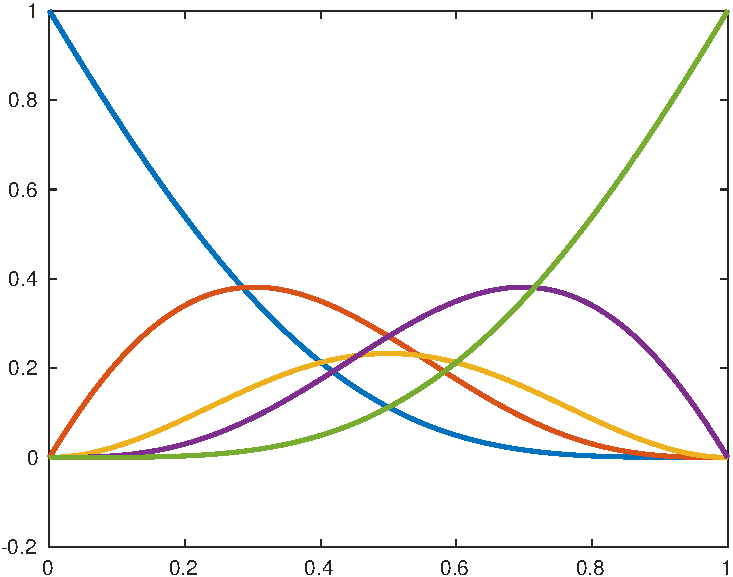
\includegraphics[width=4.5cm]{manual_ex_tbspline0}
\end{center}
\vspace*{-0.30cm}
\end{example}

%------------------------------------------------------------------

\subsection{TB\_visualization\_spline} \label{sec:matlab-tb-visualization-spline}

This function visualizes a spline in TB-spline form.

\syntax{TB\_visualization\_spline(P, cc, n, specs)}

\begin{inputlist}
  \paramitem{P}{TB-spline patch}
  \paramitem{cc}{vector of coefficients}
  \paramitem{n}{number of evaluation points (optional)}
  \paramitem{specs}{pass any number of plot specifications (optional)}
\end{inputlist}

\begin{remark}
\noindent Each element of the vector \texttt{cc} corresponds to a TB-spline basis function in the TB-spline patch. Hence, \texttt{length(cc)} should be equal to \texttt{P.n}. The parameter \texttt{n} is a positive integer scalar. When no value is specified, \texttt{n = 100} is assumed. The parameter \texttt{specs} allows for any number of input arguments, which are passed on to the function \texttt{plot}. We refer the reader to the documentation of \texttt{plot} for all the plotting options.
\end{remark}

\begin{example}
\noindent Create a TB-spline patch and a vector of coefficients, and then plot the corresponding spline in TB-spline form:
\medskip

\texttt{>> P = TB\_patch\_gtrig(4, [0, 1], 5);}

\texttt{>> cc = [1, 3, 5, 5, 2];}

\texttt{>> TB\_visualization\_spline(P, cc, 100, 'LineWidth', 2);}

\begin{center}
  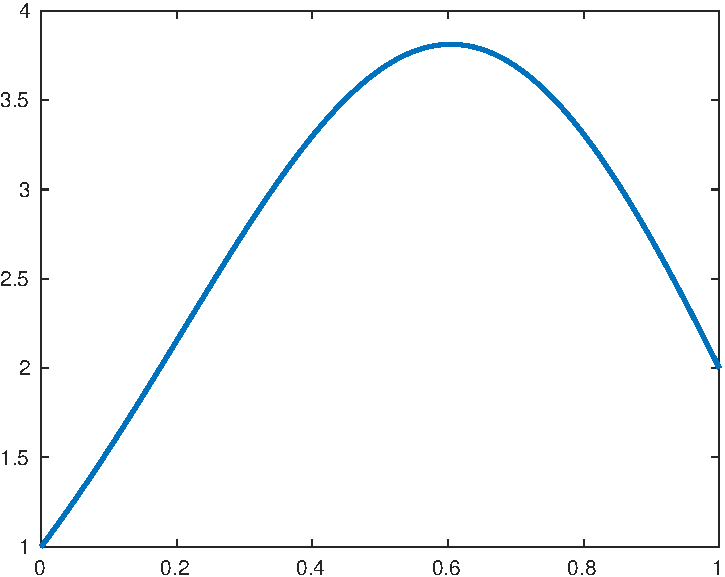
\includegraphics[width=4.5cm]{manual_ex_tbspline1}
\end{center}
\vspace*{-0.30cm}
\end{example}

%------------------------------------------------------------------

\subsection{TB\_visualization\_curve} \label{sec:matlab-tb-visualization-curve}

This function visualizes a spline curve in TB-spline form.

\syntax{TB\_visualization\_curve(P, cc, n, specs)}

\begin{inputlist}
  \paramitem{P}{TB-spline patch}
  \paramitem{cc}{matrix of control points (1D, 2D or 3D)}
  \paramitem{n}{number of evaluation points (optional)}
  \paramitem{specs}{pass any number of plot specifications (optional)}
\end{inputlist}

\begin{remark}
\noindent Each column of the matrix \texttt{cc} corresponds to a TB-spline basis function in the TB-spline patch. Hence, \texttt{size(cc,2)} should be equal to \texttt{P.n}. This matrix consists of $1$, $2$ or $3$ rows, identifying a function, a 2D curve or a 3D curve, respectively. The parameter \texttt{n} is a positive integer scalar. When no value is specified, \texttt{n = 100} is assumed. The parameter \texttt{specs} allows for any number of input arguments, which are passed on to the function \texttt{plot}/\texttt{plot3}. We refer the reader to the documentation of \texttt{plot}/\texttt{plot3} for all the plotting options.
\end{remark}

\begin{example}
\noindent Create a TB-spline patch and a matrix of 2D control points, and then plot the corresponding spline curve in TB-spline form:
\medskip

\texttt{>> P = TB\_patch\_gtrig(4, [0, 1], 5);}

\texttt{>> cc = [1, 3, 5, 3, 1; 2, 1, 3, 4, 2];}

\texttt{>> TB\_visualization\_curve(P, cc, 100, 'LineWidth', 2);}

\begin{center}
  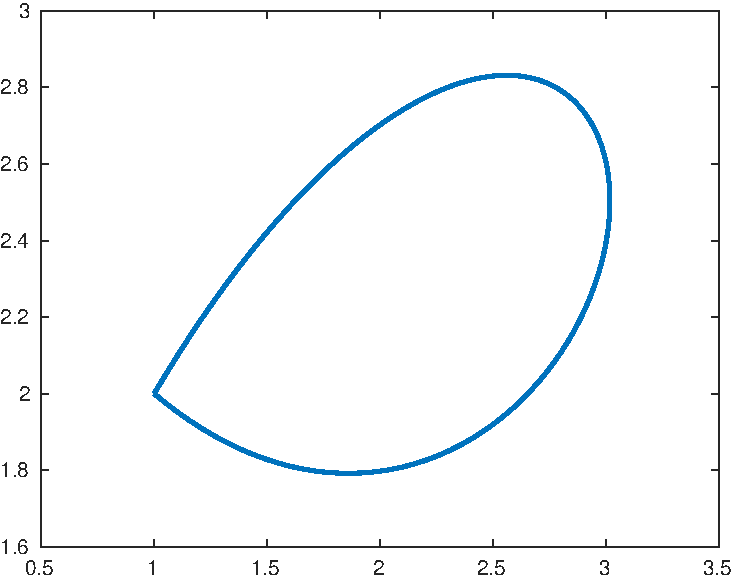
\includegraphics[width=4.5cm]{manual_ex_tbspline2}
\end{center}
\vspace*{-0.30cm}
\end{example}

%------------------------------------------------------------------

\subsection{TB\_conversion} \label{sec:matlab-tb-conversion}

This function converts a spline in TB-spline form into another TB-spline form. The conversion is exact when the source and destination TB-spline patches imply nested spaces. It is assumed that Greville points can be computed.

\syntax{ccd = TB\_conversion(Pd, Ps, ccs, sh)}

\pagebreak
\vspace*{-0.60cm}
\begin{inputlist}
  \paramitem{Pd}{destination TB-spline patch}
  \paramitem{Ps}{source TB-spline patch}
  \paramitem{ccs}{source coefficient vector}
  \paramitem{sh}{shift of the source patch (optional)}
\end{inputlist}

\begin{outputlist}
  \paramitem{ccd}{destination coefficient vector}
\end{outputlist}

\begin{remark}
\noindent Different types of TB-spline patches for \texttt{Ps} and \texttt{Pd} may be mixed. Each element of the vector \texttt{ccs} corresponds to a TB-spline basis function in the TB-spline patch \texttt{Ps}. Hence, \texttt{length(ccs)} should be equal to \texttt{Ps.n}. Similarly, each element of the resulting vector \texttt{ccd} corresponds to a TB-spline basis function in the TB-spline patch \texttt{Pd}. The parameter \texttt{sh} is a real scalar. When no value is specified, \texttt{sh = 0} is assumed.
\end{remark}

\begin{example}
\noindent Create a TB-spline patch of degree $4$ and a vector of coefficients; then, raise the degree to $9$ and compute the coefficients of the new TB-spline form:
\medskip

\texttt{>> Ps = TB\_patch\_gtrig(4, [0, 1], 5);}

\texttt{>> ccs = [1, 3, 5, 5, 2];}

\texttt{>> Pd = TB\_patch\_gtrig(9, [0, 1], 5);}

\texttt{>> ccd = TB\_conversion(Pd, Ps, ccs)}

\texttt{ccd =}

\texttt{\ \ Columns 1 through 7}

\texttt{\ \ \ \ 1.0000\ \ \ \ 1.5889\ \ \ \ 2.2889\ \ \ \ 3.0908\ \ \ \ 3.8289\ \ \ \ 4.2506\ \ \ \ 4.1879}

\texttt{\ \ Columns 8 through 10}

\texttt{\ \ \ \ 3.6730\ \ \ \ 2.8833\ \ \ \ 2.0000}

\medskip
\noindent Now, convert it into a more general TB-spline patch that is shifted by $10$:
\medskip

\texttt{>> ww = complex([0, 3], [5, 0]);}

\texttt{>> Pe = TB\_patch\_tcheb(9, [10, 11], ww, [1, 2]);}

\texttt{>> cce = TB\_conversion(Pe, Ps, ccs, 10)}


\texttt{\ \ Columns 1 through 7}

\texttt{\ \ \ \ 1.0000\ \ \ \ 1.6283\ \ \ \ 2.3704\ \ \ \ 3.2081\ \ \ \ 3.9310\ \ \ \ 4.2723\ \ \ \ 4.1184}

\texttt{\ \ Columns 8 through 10}

\texttt{\ \ \ \ 3.5658\ \ \ \ 2.8059\ \ \ \ 2.0000}

\medskip
\noindent It is no surprise that the vectors \texttt{ccd} and \texttt{cce} are similar because the corresponding basis functions look similar as well, up to the shift.
\end{example}

%------------------------------------------------------------------

\section{MDTB-spline multi-patches}\label{sec:matlab-mdtb}

The main multi-patch data-structure is called \emph{MDTB-spline multi-patch}. It contains a vector of TB-spline patches and the corresponding cumulative dimension. 

The following \Matlab{} functions are provided for constructing MDTB-spline multi-patches.
\begin{itemize}
  \item[$\bullet$] \hyperref[sec:matlab-mdtb-patch]{\texttt{MDTB\_patch}}: 
    construction of an MDTB-spline multi-patch from TB-spline segments;
  \item[$\bullet$] \hyperref[sec:matlab-mdtb-patch-tcheb]{\texttt{MDTB\_patch\_tcheb}}: 
    construction of an MDTB-spline multi-patch from Tchebycheff segments based on constant-coefficient linear differential operators; 
  \item[$\bullet$] \hyperref[sec:matlab-mdtb-patch-poly]{\texttt{MDTB\_patch\_poly}}: 
    construction of an MDTB-spline multi-patch from algebraic polynomial or algebraic polynomial spline segments; 
  \item[$\bullet$] \hyperref[sec:matlab-mdtb-patch-ppoly]{\texttt{MDTB\_patch\_ppoly}}: 
    construction of an MDTB-spline multi-patch from polynomial segments (algebraic/exponential/trigonometric); 
  \item[$\bullet$] \hyperref[sec:matlab-mdtb-patch-gpoly]{\texttt{MDTB\_patch\_gpoly}}: 
    construction of an MDTB-spline multi-patch from generalized polynomial segments (algebraic/exponential/trigonometric).
\end{itemize}
The following \Matlab{} functions are provided for core operations on MDTB-spline multi-patches.
\begin{itemize}
  \item[$\bullet$] \hyperref[sec:matlab-mdtb-extraction]{\texttt{MDTB\_extraction}}: 
    computation of the multi-degree spline extraction matrix;
  \item[$\bullet$] \hyperref[sec:matlab-mdtb-extraction-periodic]{\texttt{MDTB\_extraction\_periodic}}: 
    computation of the multi-degree spline extraction matrix with periodicity;
  \item[$\bullet$] \hyperref[sec:matlab-mdtb-extraction-local]{\texttt{MDTB\_extraction\_local}}: 
    computation of the local multi-degree spline extraction matrix corresponding to a single patch.
\end{itemize}
Furthermore, the following \Matlab{} functions are provided for working with MDTB-splines. Thanks to the multi-degree spline extraction operator, their implementation can be easily redirected to their TB-spline analogues described in Section~\ref{sec:matlab-tb}.
\begin{itemize}
  \item[$\bullet$] \hyperref[sec:matlab-mdtb-domain]{\texttt{MDTB\_domain}}: 
    computation of the end points of the domain related to a multi-patch;
  \item[$\bullet$] \hyperref[sec:matlab-mdtb-greville]{\texttt{MDTB\_greville}}: 
    computation of the multi-degree Greville points;
  \item[$\bullet$] \hyperref[sec:matlab-mdtb-evaluation-all]{\texttt{MDTB\_evaluation\_all}}: 
    evaluation of all MDTB-spline basis functions in given points;
  \item[$\bullet$] \hyperref[sec:matlab-mdtb-evaluation-spline]{\texttt{MDTB\_evaluation\_spline}}: 
    evaluation of a multi-degree spline in given points;
  \item[$\bullet$] \hyperref[sec:matlab-mdtb-evaluation-curve]{\texttt{MDTB\_evaluation\_curve}}: 
    evaluation of a multi-degree spline curve in given points;
  \item[$\bullet$] \hyperref[sec:matlab-mdtb-differentiation-all]{\texttt{MDTB\_differentiation\_all}}: 
    differentiation of all MDTB-spline basis functions in given points;
  \item[$\bullet$] \hyperref[sec:matlab-mdtb-differentiation-spline]{\texttt{MDTB\_differentiation\_spline}}: 
    differentiation of a multi-degree spline in given points;
  \item[$\bullet$] \hyperref[sec:matlab-mdtb-differentiation-curve]{\texttt{MDTB\_differentiation\_curve}}: 
    differentiation of a multi-degree spline curve in given points;
  \item[$\bullet$] \hyperref[sec:matlab-mdtb-visualization-all]{\texttt{MDTB\_visualization\_all}}: 
    visualization of all MDTB-spline basis functions;
  \item[$\bullet$] \hyperref[sec:matlab-mdtb-visualization-spline]{\texttt{MDTB\_visualization\_spline}}: 
    visualization of a multi-degree spline;
  \item[$\bullet$] \hyperref[sec:matlab-mdtb-visualization-curve]{\texttt{MDTB\_visualization\_curve}}: 
    visualization of a multi-degree spline curve;
  \item[$\bullet$] \hyperref[sec:matlab-mdtb-conversion]{\texttt{MDTB\_conversion}}: 
    conversion from source to destination MDTB-spline form.
\end{itemize}

%------------------------------------------------------------------

\subsection{MDTB\_patch} \label{sec:matlab-mdtb-patch}

This function prepares the data-structure for an MDTB-spline multi-patch, starting from a sequence of TB-spline segments. The MDTB-spline multi-patch stores a vector of TB-spline patches \texttt{P} and the corresponding cumulative dimension \texttt{mu}. 

\syntax{MP = MDTB\_patch(PP)}

\begin{inputlist}
  \paramitem{PP}{vector of B-spline patches}
\end{inputlist}

\begin{outputlist}
  \paramitem{MP}{MDTB-spline multi-patch}
\end{outputlist}

\begin{example}
\noindent Create an MDTB-spline multi-patch consisting of two TB-spline patches with different degrees ($3$ and $4$): 
\medskip

\texttt{>> P1 = TB\_patch\_gexp(3, [0, 1], 5);}

\texttt{>> P2 = TB\_patch\_gtrig(4, [1, 3], 2);}

\texttt{>> MP = MDTB\_patch([P1, P2])}

\texttt{MP = }

\texttt{\ \ \ \ P:\ [1x2 TB\_patch]}

\texttt{\ \ \ mu:\ [0 4 9]}

\texttt{>> MP.P(1)}

\texttt{ans =}

\texttt{\ \ \ \ w:\ 5}

\texttt{\ \ \ \ t:\ 1}

\texttt{\ \ \ \ m:\ 10}

\texttt{\ \ \ \ C:\ [4x4 double]}

\texttt{\ \ \ \ p:\ 3}

\texttt{\ \ \ \ n:\ 4}

\texttt{\ \ \ \ U:\ [0 1]}

\texttt{>> MP.P(2)}

\texttt{ans =}

\texttt{\ \ \ \ w:\ 2}

\texttt{\ \ \ \ t:\ 1}

\texttt{\ \ \ \ m:\ 10}

\texttt{\ \ \ \ C:\ [5x5 double]}

\texttt{\ \ \ \ p:\ 4}

\texttt{\ \ \ \ n:\ 5}

\texttt{\ \ \ \ U:\ [1 3]}    
\end{example}

%------------------------------------------------------------------

\subsection{MDTB\_patch\_tcheb} \label{sec:matlab-mdtb-patch-tcheb}

This function prepares the data-structure for an MDTB-spline multi-patch, starting from a sequence of Tchebycheff segments based on constant-coefficient linear differential operators (see \hyperref[sec:matlab-tb-patch-tcheb]{\texttt{TB\_patch\_tcheb}}). The MDTB-spline multi-patch stores a vector of TB-spline patches \texttt{P} and the corresponding cumulative dimension \texttt{mu}. 

\syntax{MP = MDTB\_patch\_tcheb(pp, xx, ww, mm)}

\begin{inputlist}
  \paramitem{pp}{vector of TB-spline degrees}
  \paramitem{xx}{vector of break points}
  \paramitem{ww}{cell array of TB-spline roots (optional)}
  \paramitem{mm}{cell array of TB-spline multiplicities (optional)}
\end{inputlist}

\begin{outputlist}
  \paramitem{MP}{MDTB-spline multi-patch}
\end{outputlist}

\begin{remark}
\noindent The parameter \texttt{xx} is a vector consisting of a strictly increasing sequence of real values (indicating the different segments). The parameter \texttt{pp} can be a scalar or a vector whose elements are non-negative integers. If \texttt{pp} is a scalar, then degree \texttt{pp} is used on each interval. On the other hand, if \texttt{pp} is a vector, then \texttt{pp(i)} is the degree on the interval \texttt{[xx(i), xx(i+1)]} for \texttt{i = 1:length(xx)-1}. Hence, \texttt{length(pp)} should be equal to \texttt{1} or \texttt{length(xx)-1}. The parameter \texttt{ww} is a cell array of vectors of roots (complex values) and the parameter \texttt{mm} is a cell array of the corresponding multiplicities (integer values). Both cell arrays should have a length equal to \texttt{1} or \texttt{length(xx)-1}. If the length is \texttt{1}, then the same root parameters are considered on each interval; otherwise, \texttt{ww\{i\}} and \texttt{mm\{i\}} are considered on the interval \texttt{[xx(i), xx(i+1)]} for \texttt{i = 1:length(xx)-1}. When no roots are specified, \texttt{ww = \{0\}} is assumed. When no multiplicities are specified, \texttt{mm = \{1\}} is assumed. We refer the reader to the documentation of \hyperref[sec:matlab-tb-patch-tcheb]{\texttt{TB\_patch\_tcheb}} for a description of how to construct a valid set of root parameters. 
\end{remark}

\begin{example}
\noindent Create an MDTB-spline multi-patch consisting of two TB-spline patches with different degrees ($3$ and $4$) by specifying the roots of the characteristic polynomials: 
\medskip

\texttt{>> ww = \{complex(1, 1), complex([0, 3], [1, 0])\};}

\texttt{>> mm = \{1, [1, 2]\};}

\texttt{>> MP = MDTB\_patch\_tcheb([3, 4], [0, 1, 3], ww, mm)}

\texttt{MP = }

\texttt{\ \ \ \ P:\ [1x2 TB\_patch\_tcheb]}

\texttt{\ \ \ mu:\ [0 4 9]}

\pagebreak

\texttt{>> MP.P(1)}

\texttt{ans =}

\texttt{\ \ \ \ W:\ [2x4 double]}

\texttt{\ \ \ mu:\ [0 2 4]}

\texttt{\ \ \ \ C:\ [4x4 double]}

\texttt{\ \ \ \ p:\ 3}

\texttt{\ \ \ \ n:\ 4}

\texttt{\ \ \ \ U:\ [0 1]}

\texttt{>> MP.P(2)}

\texttt{ans =}

\texttt{\ \ \ \ W:\ [3x4 double]}

\texttt{\ \ \ mu:\ [0 1 3 5]}

\texttt{\ \ \ \ C:\ [5x5 double]}

\texttt{\ \ \ \ p:\ 4}

\texttt{\ \ \ \ n:\ 5}

\texttt{\ \ \ \ U:\ [1 3]}    
\end{example}

%------------------------------------------------------------------

\subsection{MDTB\_patch\_poly} \label{sec:matlab-mdtb-patch-poly}

This function prepares the data-structure for an MDTB-spline multi-patch, starting from a sequence of algebraic polynomial segments and smoothness relations. The MDTB-spline multi-patch stores a vector of TB-spline patches \texttt{P} and the corresponding cumulative dimension \texttt{mu}. Consecutive polynomial segments of the same degree are merged into a single TB-spline patch, unless specified otherwise (see \hyperref[sec:matlab-tb-patch-poly]{\texttt{TB\_patch\_poly}} and \hyperref[sec:matlab-tb-patch-spline]{\texttt{TB\_patch\_spline}}).

\syntax{[MP, rr] = MDTB\_patch\_poly(pp, xx, kk, mg)}

\begin{inputlist}
  \paramitem{pp}{vector of polynomial degrees}
  \paramitem{xx}{vector of break points}
  \paramitem{kk}{smoothness vector (optional)}
  \paramitem{mg}{same degree merged if true (optional)}
\end{inputlist}

\begin{outputlist}
  \paramitem{MP}{MDTB-spline multi-patch}
  \paramitem{rr}{MDTB-spline smoothness vector (optional)}
\end{outputlist}

\begin{remark}
\noindent The parameter \texttt{xx} is a vector consisting of a strictly increasing sequence of real values (indicating the different segments). The parameter \texttt{pp} can be a scalar or a vector whose elements are non-negative integers. If \texttt{pp} is a scalar, then degree \texttt{pp} is used on each interval. On the other hand, if \texttt{pp} is a vector, then \texttt{pp(i)} is the degree on the interval \linebreak \texttt{[xx(i), xx(i+1)]} for \texttt{i = 1:length(xx)-1}. Hence, \texttt{length(pp)} should be equal to \texttt{1} or \texttt{length(xx)-1}. The parameter \texttt{kk} can be a scalar or a vector whose elements are non-negative integers. If \texttt{kk} is a scalar, then \texttt{kk} should be less than \texttt{min(pp)}, and smoothness \texttt{kk} is imposed at the break point \texttt{xx(i+1)} for \texttt{i = 1:length(xx)-2}. On the other hand, if \texttt{kk} is a vector, then \texttt{kk(i)} should be less than \texttt{min(pp(i),pp(i+1))}, and smoothness \texttt{kk(i)} is imposed at the break point \texttt{xx(i+1)} for \texttt{i = 1:length(xx)-2}. Hence, \texttt{length(kk)} should be equal to \texttt{1} or \texttt{length(xx)-2}. When no smoothness is specified, \texttt{kk = 0} is assumed. The parameter \texttt{mg} is a boolean scalar. If \texttt{mg} is \texttt{true}, then consecutive polynomial segments of the same degree are merged into a single polynomial TB-spline patch; otherwise, they are not merged. When no value is specified, \texttt{mg = true} is assumed. The resulting vector \texttt{rr} represents the corresponding smoothness between the TB-spline patches, so \texttt{length(rr)} equals \texttt{length(MP.P)-1}.
\end{remark}

\begin{example}
\noindent Create an MDTB-spline multi-patch consisting of four polynomial segments with different degrees ($3$ and $4$) that are connected with smoothness $C^2$: 
\medskip

\texttt{>> [MP, rr] = MDTB\_patch\_poly([3, 3, 4, 4], [0, 1, 3, 4, 6], 2)}

\texttt{MP = }

\texttt{\ \ \ \ P:\ [1x2 TB\_patch\_spline]}

\texttt{\ \ \ mu:\ [0 5 12]}

\texttt{rr = }

\texttt{\ \ \ \ 2}

\texttt{>> MP.P(1)}

\texttt{ans =}

\texttt{\ \ \ \ p:\ 3}

\texttt{\ \ \ \ n:\ 5}

\texttt{\ \ \ \ U:\ [0 0 0 0 1 3 3 3 3]}

\texttt{>> MP.P(2)}

\texttt{ans =}

\texttt{\ \ \ \ p:\ 4}

\texttt{\ \ \ \ n:\ 7}

\texttt{\ \ \ \ U:\ [3 3 3 3 3 4 4 6 6 6 6 6]}    
\end{example}

%------------------------------------------------------------------

\subsection{MDTB\_patch\_ppoly} \label{sec:matlab-mdtb-patch-ppoly}

This function prepares the data-structure for an MDTB-spline multi-patch, starting from a sequence of polynomial-type segments. There are three types of segments:
\begin{itemize}
  \item[$\bullet$] type 0: algebraic (see \hyperref[sec:matlab-tb-patch-poly]{\texttt{TB\_patch\_poly}});
  \item[$\bullet$] type 1: exponential (see \hyperref[sec:matlab-tb-patch-pexp]{\texttt{TB\_patch\_pexp}});
  \item[$\bullet$] type 2: trigonometric (see \hyperref[sec:matlab-tb-patch-ptrig]{\texttt{TB\_patch\_ptrig}}).
\end{itemize}
The MDTB-spline multi-patch stores a vector of TB-spline patches \texttt{P} and the corresponding cumulative dimension \texttt{mu}. 

\pagebreak
\syntax{MP = MDTB\_patch\_ppoly(pp, xx, tp, ww)}

\begin{inputlist}
  \paramitem{pp}{vector of TB-spline degrees}
  \paramitem{xx}{vector of break points}
  \paramitem{tp}{vector of TB-spline types (optional)}
  \paramitem{ww}{vector of TB-spline parameters (optional)}
\end{inputlist}

\begin{outputlist}
  \paramitem{MP}{MDTB-spline multi-patch}
\end{outputlist}

\begin{remark}
\noindent The parameter \texttt{xx} is a vector consisting of a strictly increasing sequence of real values (indicating the different segments). The parameter \texttt{pp} can be a scalar or a vector whose elements are non-negative integers. If \texttt{pp} is a scalar, then degree \texttt{pp} is used on each interval. On the other hand, if \texttt{pp} is a vector, then \texttt{pp(i)} is the degree on the interval \texttt{[xx(i), xx(i+1)]} for \texttt{i = 1:length(xx)-1}. Hence, \texttt{length(pp)} should be equal to \texttt{1} or \texttt{length(xx)-1}. The parameter \texttt{tp} can be a scalar or a vector whose elements are \texttt{0}, \texttt{1} or \texttt{2}. If \texttt{tp} is a scalar, then TB-spline type \texttt{tp} is used on each interval. On the other hand, if \texttt{tp} is a vector, then \texttt{tp(i)} is the TB-spline type on the interval \texttt{[xx(i), xx(i+1)]} for \texttt{i = 1:length(xx)-1}. Hence, \texttt{length(tp)} should be equal to \texttt{1} or \texttt{length(xx)-1}. When no value is specified, \texttt{tp = 0} is assumed.
The parameter \texttt{ww} can be a scalar or a vector of TB-spline type-specific parameters. If \texttt{ww} is a scalar, then the same value is considered on each interval; otherwise, \texttt{ww(i)} is considered on the interval \texttt{[xx(i), xx(i+1)]} for \texttt{i~= 1:length(xx)-1}. Hence, \texttt{length(ww)} should be equal to \texttt{1} or \texttt{length(xx)-1}.
In the case of exponential and trigonometric segments, we refer the reader to the documentation of \hyperref[sec:matlab-tb-patch-pexp]{\texttt{TB\_patch\_pexp}} and \hyperref[sec:matlab-tb-patch-ptrig]{\texttt{TB\_patch\_ptrig}} for a description of these type-specific parameters and their default values. In the case of algebraic polynomial segments, these parameters have no meaning and can be set arbitrarily.
\end{remark}

\begin{example}
\noindent Create an MDTB-spline multi-patch consisting of two polynomial-type segments with different degrees ($2$ and $4$): 
\medskip

\texttt{>> MP = MDTB\_patch\_ppoly([2, 4], [0, 1, 3], [1, 2], [5, 1])}

\texttt{MP = }

\texttt{\ \ \ \ P:\ [1x2 TB\_patch\_poly]}

\texttt{\ \ \ mu:\ [0 3 8]}

\texttt{>> MP.P(1)}

\texttt{ans =}

\texttt{\ \ \ \ w:\ 5}

\texttt{\ \ \ ss:\ [3x1 double]}

\texttt{\ \ \ \ p:\ 2}

\texttt{\ \ \ \ n:\ 3}

\texttt{\ \ \ \ U:\ [0 1]}

\pagebreak

\texttt{>> MP.P(2)}

\texttt{ans =}

\texttt{\ \ \ \ w:\ 1}

\texttt{\ \ \ ss:\ [5x1 double]}

\texttt{\ \ \ \ p:\ 4}

\texttt{\ \ \ \ n:\ 5}

\texttt{\ \ \ \ U:\ [1 3]}    
\end{example}

%------------------------------------------------------------------

\subsection{MDTB\_patch\_gpoly} \label{sec:matlab-mdtb-patch-gpoly}

This function prepares the data-structure for an MDTB-spline multi-patch, starting from a sequence of generalized polynomial segments. There are three types of segments:
\begin{itemize}
  \item[$\bullet$] type 0: algebraic (see \hyperref[sec:matlab-tb-patch-poly]{\texttt{TB\_patch\_poly}});
  \item[$\bullet$] type 1: exponential (see \hyperref[sec:matlab-tb-patch-gexp]{\texttt{TB\_patch\_gexp}});
  \item[$\bullet$] type 2: trigonometric (see \hyperref[sec:matlab-tb-patch-gtrig]{\texttt{TB\_patch\_gtrig}}).
\end{itemize}
The MDTB-spline multi-patch stores a vector of TB-spline patches \texttt{P} and the corresponding cumulative dimension \texttt{mu}. 

\syntax{MP = MDTB\_patch\_gpoly(pp, xx, tp, ww, tt, mm)}

\begin{inputlist}
  \paramitem{pp}{vector of TB-spline degrees}
  \paramitem{xx}{vector of break points}
  \paramitem{tp}{vector of TB-spline types (optional)}
  \paramitem{ww}{vector of TB-spline parameters (optional)}
  \paramitem{tt}{vector of representation types (optional)}
  \paramitem{mm}{vector of representation parameters (optional)}
\end{inputlist}

\begin{outputlist}
  \paramitem{MP}{MDTB-spline multi-patch}
\end{outputlist}

\begin{remark}
\noindent The parameter \texttt{xx} is a vector consisting of a strictly increasing sequence of real values (indicating the different segments). The parameter \texttt{pp} can be a scalar or a vector whose elements are non-negative integers. If \texttt{pp} is a scalar, then degree \texttt{pp} is used on each interval. On the other hand, if \texttt{pp} is a vector, then \texttt{pp(i)} is the degree on the interval \texttt{[xx(i), xx(i+1)]} for \texttt{i = 1:length(xx)-1}. Hence, \texttt{length(pp)} should be equal to \texttt{1} or \texttt{length(xx)-1}. The parameter \texttt{tp} can be a scalar or a vector whose elements are \texttt{0}, \texttt{1} or \texttt{2}. If \texttt{tp} is a scalar, then TB-spline type \texttt{tp} is used on each interval. On the other hand, if \texttt{tp} is a vector, then \texttt{tp(i)} is the TB-spline type on the interval \texttt{[xx(i), xx(i+1)]} for \texttt{i = 1:length(xx)-1}. Hence, \texttt{length(tp)} should be equal to \texttt{1} or \texttt{length(xx)-1}. When no value is specified, \texttt{tp = 0} is assumed.
The parameters \texttt{ww}, \texttt{tt} and \texttt{mm} can be scalars or vectors of TB-spline type-specific parameters. If they are scalars, then the same values are considered on each interval; otherwise, \texttt{ww(i)}, \texttt{tt(i)} and \texttt{mm(i)} are considered on the interval \texttt{[xx(i), xx(i+1)]} for \texttt{i = 1:length(xx)-1}. Hence, their length should be equal to \texttt{1} or \texttt{length(xx)-1}.
In the case of exponential and trigonometric segments, we refer the reader to the documentation of \hyperref[sec:matlab-tb-patch-gexp]{\texttt{TB\_patch\_gexp}} and \hyperref[sec:matlab-tb-patch-gtrig]{\texttt{TB\_patch\_gtrig}} for a description of these type-specific parameters and their default values. In the case of algebraic polynomial segments, these parameters have no meaning and can be set arbitrarily.
\end{remark}

\begin{example}
\noindent Create an MDTB-spline multi-patch consisting of two generalized polynomial segments with different degrees ($3$ and $4$): 
\medskip

\texttt{>> MP = MDTB\_patch\_gpoly([3, 4], [0, 1, 3], [1, 2], [5, 2])}

\texttt{MP = }

\texttt{\ \ \ \ P:\ [1x2 TB\_patch]}

\texttt{\ \ \ mu:\ [0 4 9]}

\texttt{>> MP.P(1)}

\texttt{ans =}

\texttt{\ \ \ \ w:\ 5}

\texttt{\ \ \ \ t:\ 1}

\texttt{\ \ \ \ m:\ 10}

\texttt{\ \ \ \ C:\ [4x4 double]}

\texttt{\ \ \ \ p:\ 3}

\texttt{\ \ \ \ n:\ 4}

\texttt{\ \ \ \ U:\ [0 1]}

\texttt{>> MP.P(2)}

\texttt{ans =}

\texttt{\ \ \ \ w:\ 2}

\texttt{\ \ \ \ t:\ 1}

\texttt{\ \ \ \ m:\ 10}

\texttt{\ \ \ \ C:\ [5x5 double]}

\texttt{\ \ \ \ p:\ 4}

\texttt{\ \ \ \ n:\ 5}

\texttt{\ \ \ \ U:\ [1 3]}    
\end{example}

%------------------------------------------------------------------

\subsection{MDTB\_extraction} \label{sec:matlab-mdtb-extraction}

This function computes the multi-degree spline extraction matrix representing a set of MDTB-spline basis functions in terms of the TB-spline basis functions related to a given sequence of TB-spline patches.

\syntax{H = MDTB\_extraction(MP, rr)}

\pagebreak
\vspace*{-0.60cm}
\begin{inputlist}
  \paramitem{MP}{MDTB-spline multi-patch}
  \paramitem{rr}{MDTB-spline smoothness vector (optional)}
\end{inputlist}

\begin{outputlist}
  \paramitem{H}{extraction matrix}
\end{outputlist}

\begin{remark}
\noindent The parameter \texttt{rr} can be a scalar or a vector whose elements are integers.
If \texttt{rr} is a scalar, then \texttt{rr} should be less than \texttt{min([MP.P.p])}, and smoothness \texttt{rr} is imposed between all consecutive TB-spline patches. On the other hand, if \texttt{rr} is a vector, then \texttt{rr(i)} should be less than \texttt{min(MP.P(i).p,MP.P(i+1).p)}, and smoothness \texttt{rr(i)} is imposed between TB-spline patches \texttt{MP.P(i)} and \texttt{MP.P(i+1)} for \texttt{i = 1:length(MP.P)-1}.
Hence, \texttt{length(rr)} should be equal to \texttt{1} or \texttt{length(MP.P)-1}. 
A negative value indicates no active smoothness imposition.
When no smoothness is specified, \texttt{rr = 0} is assumed. 
The resulting matrix \texttt{H} is encoded in sparse format;
each row in \texttt{H} corresponds to an MDTB-spline basis function and each column to a TB-spline basis function in one of the TB-spline patches, so \texttt{size(H,2)} equals \texttt{MP.mu(end)}.
\end{remark}

\begin{example}
\noindent Create an MDTB-spline multi-patch and compute the multi-degree spline extraction matrix for a given smoothness pattern:
\medskip

\texttt{>> MP = MDTB\_patch\_gpoly([3, 4], [0, 1, 3], [1, 2], [5, 2]);}

\texttt{>> H = MDTB\_extraction(MP, 2);}

\texttt{>> Hfull = full(H)}

\texttt{Hfull =}

\texttt{\ \ Columns 1 through 7}

\texttt{\ \ \ \ 1.0000\ \ \ \ \ \ \ \ \ 0\ \ \ \ \ \ \ \ \ 0\ \ \ \ \ \ \ \ \ 0\ \ \ \ \ \ \ \ \ 0\ \ \ \ \ \ \ \ \ 0\ \ \ \ \ \ \ \ \ 0}

\texttt{\ \ \ \ \ \ \ \ \ 0\ \ \ \ 1.0000\ \ \ \ 0.5476\ \ \ \ 0.4267\ \ \ \ 0.4267\ \ \ \ \ \ \ \ \ 0\ \ \ \ \ \ \ \ \ 0}

\texttt{\ \ \ \ \ \ \ \ \ 0\ \ \ \ \ \ \ \ \ 0\ \ \ \ 0.4524\ \ \ \ 0.5210\ \ \ \ 0.5210\ \ \ \ 0.7632\ \ \ \ \ \ \ \ \ 0}

\texttt{\ \ \ \ \ \ \ \ \ 0\ \ \ \ \ \ \ \ \ 0\ \ \ \ \ \ \ \ \ 0\ \ \ \ 0.0523\ \ \ \ 0.0523\ \ \ \ 0.2368\ \ \ \ 1.0000}

\texttt{\ \ \ \ \ \ \ \ \ 0\ \ \ \ \ \ \ \ \ 0\ \ \ \ \ \ \ \ \ 0\ \ \ \ \ \ \ \ \ 0\ \ \ \ \ \ \ \ \ 0\ \ \ \ \ \ \ \ \ 0\ \ \ \ \ \ \ \ \ 0}

\texttt{\ \ \ \ \ \ \ \ \ 0\ \ \ \ \ \ \ \ \ 0\ \ \ \ \ \ \ \ \ 0\ \ \ \ \ \ \ \ \ 0\ \ \ \ \ \ \ \ \ 0\ \ \ \ \ \ \ \ \ 0\ \ \ \ \ \ \ \ \ 0}

\texttt{\ \ Columns 8 through 9}

\texttt{\ \ \ \ \ \ \ \ \ 0\ \ \ \ \ \ \ \ \ 0}

\texttt{\ \ \ \ \ \ \ \ \ 0\ \ \ \ \ \ \ \ \ 0}

\texttt{\ \ \ \ \ \ \ \ \ 0\ \ \ \ \ \ \ \ \ 0}

\texttt{\ \ \ \ \ \ \ \ \ 0\ \ \ \ \ \ \ \ \ 0}

\texttt{\ \ \ \ 1.0000\ \ \ \ \ \ \ \ \ 0}

\texttt{\ \ \ \ \ \ \ \ \ 0\ \ \ \ 1.0000}
\end{example}

%------------------------------------------------------------------

\subsection{MDTB\_extraction\_periodic} \label{sec:matlab-mdtb-extraction-periodic}

This function computes the periodic multi-degree spline extraction matrix representing a set of periodic MDTB-spline basis functions in terms of the TB-spline basis functions related to a given sequence of TB-spline patches.

\syntax{H = MDTB\_extraction\_periodic(MP, rr, rp)}

\begin{inputlist}
  \paramitem{MP}{MDTB-spline multi-patch}
  \paramitem{rr}{MDTB-spline smoothness vector (optional)}
  \paramitem{rp}{periodicity smoothness (optional)}
\end{inputlist}

\begin{outputlist}
  \paramitem{H}{extraction matrix}
\end{outputlist}

\begin{remark}
\noindent The parameter \texttt{rr} can be a scalar or a vector whose elements are integers. If \texttt{rr} is a scalar, then \texttt{rr} should be less than \texttt{min([MP.P.p])}, and smoothness \texttt{rr} is imposed between all consecutive TB-spline patches. On the other hand, if \texttt{rr} is a vector, then \texttt{rr(i)} should be less than \texttt{min(MP.P(i).p,MP.P(i+1).p)}, and smoothness \texttt{rr(i)} is imposed between TB-spline patches \texttt{MP.P(i)} and \texttt{MP.P(i+1)} for \texttt{i = 1:length(MP.P)-1}. Hence, \texttt{length(rr)} should be equal to \texttt{1} or \texttt{length(MP.P)-1}. A negative value indicates no active smoothness imposition. When no smoothness is specified, \texttt{rr = 0} is assumed. The parameter \texttt{rp} should be an integer scalar less than half the dimension (floored) of the related non-periodic MDTB-spline space. When no periodicity smoothness is specified, \texttt{rp = -1} is assumed. The resulting matrix \texttt{H} is encoded in sparse format; each row in \texttt{H} corresponds to a periodic MDTB-spline basis function and each column to a TB-spline basis function in one of the TB-spline patches, so \texttt{size(H,2)} equals \texttt{MP.mu(end)}.
\end{remark}

\begin{example}
\noindent Create an MDTB-spline multi-patch and compute the periodic multi-degree spline extraction matrix for a given smoothness pattern:
\medskip

\texttt{>> MP = MDTB\_patch\_gpoly([3, 4], [0, 1, 3], [1, 2], [5, 2]);}

\texttt{>> Hper = MDTB\_extraction\_periodic(MP, 2, 1);}

\texttt{>> Hfull = full(Hper)}

\texttt{Hfull =}

\texttt{\ \ Columns 1 through 7}

\texttt{\ \ \ \ 0.2208\ \ \ \ \ \ \ \ \ 0\ \ \ \ \ \ \ \ \ 0\ \ \ \ \ \ \ \ \ 0\ \ \ \ \ \ \ \ \ 0\ \ \ \ \ \ \ \ \ 0\ \ \ \ \ \ \ \ \ 0}

\texttt{\ \ \ \ 0.7792\ \ \ \ 1.0000\ \ \ \ 0.5476\ \ \ \ 0.4267\ \ \ \ 0.4267\ \ \ \ \ \ \ \ \ 0\ \ \ \ \ \ \ \ \ 0}

\texttt{\ \ \ \ \ \ \ \ \ 0\ \ \ \ \ \ \ \ \ 0\ \ \ \ 0.4524\ \ \ \ 0.5210\ \ \ \ 0.5210\ \ \ \ 0.7632\ \ \ \ \ \ \ \ \ 0}

\texttt{\ \ \ \ \ \ \ \ \ 0\ \ \ \ \ \ \ \ \ 0\ \ \ \ \ \ \ \ \ 0\ \ \ \ 0.0523\ \ \ \ 0.0523\ \ \ \ 0.2368\ \ \ \ 1.0000}

\pagebreak

\texttt{\ \ Columns 8 through 9}

\texttt{\ \ \ \ 1.0000\ \ \ \ 0.2208}

\texttt{\ \ \ \ \ \ \ \ \ 0\ \ \ \ 0.7792}

\texttt{\ \ \ \ \ \ \ \ \ 0\ \ \ \ \ \ \ \ \ 0}

\texttt{\ \ \ \ \ \ \ \ \ 0\ \ \ \ \ \ \ \ \ 0}
\end{example}

%------------------------------------------------------------------

\subsection{MDTB\_extraction\_local} \label{sec:matlab-mdtb-extraction-local}

This function returns the local extraction matrix corresponding to a single TB-spline patch.

\syntax{Hl = MDTB\_extraction\_local(MP, H, ip)}

\begin{inputlist}
  \paramitem{MP}{MDTB-spline multi-patch}
  \paramitem{H}{extraction matrix}
  \paramitem{ip}{index of patch}
\end{inputlist}

\begin{outputlist}
  \paramitem{Hl}{local extraction matrix}
\end{outputlist}

\begin{remark}
\noindent The extraction matrix \texttt{H} should be deduced from the MDTB-spline multi-patch \texttt{MP} and incorporates the smoothness. The parameter \texttt{ip} takes an integer value between $1$ and \texttt{length(MP.P)}. The resulting matrix \texttt{Hl} is encoded in sparse format; each row in \texttt{Hl} corresponds to an MDTB-spline basis function and each column to a TB-spline basis function in the selected TB-spline patch, so \texttt{size(Hl)} equals \texttt{[size(H,1), MP.P(ip).n]}.~
\end{remark}

\begin{example}
\noindent Create an MDTB-spline multi-patch with smoothness and show the B\'ezier extraction matrix corresponding to the first patch:
\medskip

\texttt{>> MP = MDTB\_patch\_gpoly([3, 4], [0, 1, 3], [1, 2], [5, 2]);}

\texttt{>> H = MDTB\_extraction(MP, 2);}

\texttt{>> Hl = MDTB\_extraction\_local(MP, H, 1);}

\texttt{>> B = full(Hl(any(Hl, 2), :))}

\texttt{B =}

\texttt{\ \ \ \ 1.0000\ \ \ \ \ \ \ \ \ 0\ \ \ \ \ \ \ \ \ 0\ \ \ \ \ \ \ \ \ 0}

\texttt{\ \ \ \ \ \ \ \ \ 0\ \ \ \ 1.0000\ \ \ \ 0.5476\ \ \ \ 0.4267}

\texttt{\ \ \ \ \ \ \ \ \ 0\ \ \ \ \ \ \ \ \ 0\ \ \ \ 0.4524\ \ \ \ 0.5210}

\texttt{\ \ \ \ \ \ \ \ \ 0\ \ \ \ \ \ \ \ \ 0\ \ \ \ \ \ \ \ \ 0\ \ \ \ 0.0523}
\end{example}

%------------------------------------------------------------------

\subsection{MDTB\_domain} \label{sec:matlab-mdtb-domain}

This function computes the end points of the domain specified by a given MDTB-spline multi-patch. 

\syntax{[a, b] = MDTB\_domain(MP)}

\begin{inputlist}
  \paramitem{MP}{MDTB-spline multi-patch}
\end{inputlist}

\begin{outputlist}
  \paramitem{a}{left end point}
  \paramitem{b}{right end point}
\end{outputlist}

\begin{example}
\noindent Create an MDTB-spline multi-patch and show the end points of its domain:
\medskip

\texttt{>> MP = MDTB\_patch\_gpoly([3, 4], [0, 1, 3], [1, 2], [5, 2]);}

\texttt{>> [a, b] = MDTB\_domain(MP)}

\texttt{a =}

\texttt{\ \ \ \ 0}

\texttt{b =}

\texttt{\ \ \ \ 3}
\end{example}

%------------------------------------------------------------------

\subsection{MDTB\_greville} \label{sec:matlab-mdtb-greville}

This function computes the Greville points of a given MDTB-spline multi-patch with smoothness, i.e., the coefficients of the MDTB-spline form of the identity function (if possible).

\syntax{gg = MDTB\_greville(MP, H)}

\begin{inputlist}
  \paramitem{MP}{MDTB-spline multi-patch}
  \paramitem{H}{extraction matrix}
\end{inputlist}

\begin{outputlist}
  \paramitem{gg}{vector of Greville points}
\end{outputlist}

\begin{remark}
\noindent The extraction matrix \texttt{H} should be deduced from the MDTB-spline multi-patch \texttt{MP} and incorporates the smoothness. Each element of the vector \texttt{gg} corresponds to an MDTB-spline basis function, so \texttt{length(gg)} equals \texttt{size(H,1)}.
\end{remark}

\pagebreak
\vspace*{-0.45cm}
\begin{example}
\noindent Create an MDTB-spline multi-patch with smoothness and show its Greville points:
\medskip

\texttt{>> MP = MDTB\_patch\_gpoly([3, 4], [0, 1, 3], [1, 2], [5, 2]);}

\texttt{>> H = MDTB\_extraction(MP, 2);}

\texttt{>> gg = MDTB\_greville(MP, H)}

\texttt{gg =}

\texttt{\ \ \ \ 0.0000\ \ \ \ 0.1891\ \ \ \ 1.5638\ \ \ \ 2.0000\ \ \ \ 2.3329\ \ \ \ 3.0000}
\end{example}

%------------------------------------------------------------------

\subsection{MDTB\_evaluation\_all} \label{sec:matlab-mdtb-evaluation-all}

This function evaluates all (periodic) MDTB-spline basis functions of an MDTB-spline multi-patch with smoothness at a given set of points, and stores the corresponding values in a matrix.

\syntax{M = MDTB\_evaluation\_all(MP, H, xx)}

\begin{inputlist}
  \paramitem{MP}{MDTB-spline multi-patch}
  \paramitem{H}{extraction matrix}
  \paramitem{xx}{vector of evaluation points}
\end{inputlist}

\begin{outputlist}
  \paramitem{M}{evaluation matrix}
\end{outputlist}

\begin{remark}
\noindent The extraction matrix \texttt{H} should be deduced from the MDTB-spline multi-patch \texttt{MP} and incorporates the smoothness. Each row in the resulting matrix \texttt{M} corresponds to an MDTB-spline basis function and each column to an evaluation point, so \texttt{size(M)} equals \texttt{[size(H,1), length(xx)]}.
\end{remark}

\begin{example}
\noindent Create an MDTB-spline multi-patch with smoothness and evaluate all the corresponding MDTB-spline basis functions at five uniform points in the domain:
\medskip

\texttt{>> MP = MDTB\_patch\_gpoly([3, 4], [0, 1, 3], [1, 2], [5, 2]);}

\texttt{>> H = MDTB\_extraction(MP, 2);}

\texttt{>> M = MDTB\_evaluation\_all(MP, H, [1/2, 1, 3/2, 2, 5/2])}

\texttt{M =}

\texttt{\ \ \ \ 0.0513\ \ \ \ \ \ \ \ \ 0\ \ \ \ \ \ \ \ \ 0\ \ \ \ \ \ \ \ \ 0\ \ \ \ \ \ \ \ \ 0}

\texttt{\ \ \ \ 0.7163\ \ \ \ 0.4267\ \ \ \ 0.1688\ \ \ \ 0.0393\ \ \ \ 0.0027}

\texttt{\ \ \ \ 0.2297\ \ \ \ 0.5210\ \ \ \ 0.4986\ \ \ \ 0.2434\ \ \ \ 0.0417}

\texttt{\ \ \ \ 0.0027\ \ \ \ 0.0523\ \ \ \ 0.2760\ \ \ \ 0.3693\ \ \ \ 0.1768}

\texttt{\ \ \ \ \ \ \ \ \ 0\ \ \ \ 0.0000\ \ \ \ 0.0503\ \ \ \ 0.2561\ \ \ \ 0.3833}

\texttt{\ \ \ \ \ \ \ \ \ 0\ \ \ \ \ \ \ \ \ 0\ \ \ \ 0.0064\ \ \ \ 0.0920\ \ \ \ 0.3955}

\pagebreak

\noindent Now, do the same with periodic MDTB-spline basis functions:
\medskip

\texttt{>> Hper = MDTB\_extraction\_periodic(MP, 2, 1);}

\texttt{>> Mper = MDTB\_evaluation\_all(MP, Hper, [1/2, 1, 3/2, 2, 5/2])}

\texttt{Mper =}

\texttt{\ \ \ \ 0.0113\ \ \ \ 0.0000\ \ \ \ 0.0517\ \ \ \ 0.2764\ \ \ \ 0.4706}

\texttt{\ \ \ \ 0.7563\ \ \ \ 0.4267\ \ \ \ 0.1737\ \ \ \ 0.1109\ \ \ \ 0.3109}

\texttt{\ \ \ \ 0.2297\ \ \ \ 0.5210\ \ \ \ 0.4986\ \ \ \ 0.2434\ \ \ \ 0.0417}

\texttt{\ \ \ \ 0.0027\ \ \ \ 0.0523\ \ \ \ 0.2760\ \ \ \ 0.3693\ \ \ \ 0.1768}
\end{example}

%------------------------------------------------------------------

\subsection{MDTB\_evaluation\_spline} \label{sec:matlab-mdtb-evaluation-spline}

This function evaluates a spline in (periodic) MDTB-spline form at a given set of points, and stores the corresponding values in a vector.

\syntax{ss = MDTB\_evaluation\_spline(MP, H, cc, xx)}

\begin{inputlist}
  \paramitem{MP}{MDTB-spline multi-patch}
  \paramitem{H}{extraction matrix}
  \paramitem{cc}{vector of coefficients}
  \paramitem{xx}{vector of evaluation points}
\end{inputlist}

\begin{outputlist}
  \paramitem{ss}{vector of spline values}
\end{outputlist}

\begin{remark}
\noindent The extraction matrix \texttt{H} should be deduced from the MDTB-spline multi-patch \texttt{MP} and incorporates the smoothness. Each element of the vector \texttt{cc} corresponds to an MDTB-spline basis function. Hence, \texttt{length(cc)} should be equal to \texttt{size(H,1)}. Each element of the resulting vector \texttt{ss} corresponds to an evaluation point, so \texttt{length(ss)} equals \texttt{length(xx)}.
\end{remark}

\begin{example}
\noindent Create an MDTB-spline multi-patch with smoothness and a vector of coefficients, and then evaluate the corresponding spline in MDTB-spline form at three uniform points in the domain:
\medskip

\texttt{>> MP = MDTB\_patch\_gpoly([3, 4], [0, 1, 3], [1, 2], [5, 2]);}

\texttt{>> H = MDTB\_extraction(MP, 2);}

\texttt{>> cc = [1, 3, 5, 4, 0, 2];}

\texttt{>> ss = MDTB\_evaluation\_spline(MP, H, cc, [1/2, 3/2, 5/2])}

\texttt{ss =}

\texttt{\ \ \ \ 3.3595\ \ \ \ 4.1159\ \ \ \ 1.7149}

\medskip
\noindent Now, do the same with periodic MDTB-spline basis functions:
\medskip

\texttt{>> Hper = MDTB\_extraction\_periodic(MP, 2, 1);}

\texttt{>> ccper = [1, 3, 5, 4];}

\texttt{>> ssper = MDTB\_evaluation\_spline(MP, Hper, ccper, [1/2, 3/2, 5/2])}

\texttt{ssper =}

\texttt{\ \ \ \ 3.4394\ \ \ \ 4.1697\ \ \ \ 2.3190}
\end{example}

%------------------------------------------------------------------

\subsection{MDTB\_evaluation\_curve} \label{sec:matlab-mdtb-evaluation-curve}

This function evaluates a spline curve in (periodic) MDTB-spline form at a given set of points, and stores the corresponding curve points in a matrix.

\syntax{ss = MDTB\_evaluation\_curve(MP, H, cc, xx)}

\begin{inputlist}
  \paramitem{MP}{MDTB-spline multi-patch}
  \paramitem{H}{extraction matrix}
  \paramitem{cc}{matrix of control points (1D, 2D or 3D)}
  \paramitem{xx}{vector of evaluation points}
\end{inputlist}

\begin{outputlist}
  \paramitem{ss}{matrix of spline curve points}
\end{outputlist}

\begin{remark}
\noindent The extraction matrix \texttt{H} should be deduced from the MDTB-spline multi-patch \texttt{MP} and incorporates the smoothness. Each column of the matrix \texttt{cc} corresponds to an MDTB-spline basis function. Hence, \texttt{size(cc,2)} should be equal to \texttt{size(H,1)}. This matrix consists of $1$, $2$ or $3$ rows, identifying a function, a 2D curve or a 3D curve, respectively. Each column of the resulting matrix \texttt{ss} corresponds to an evaluation point and this matrix has the same number of rows as \texttt{cc}, so \texttt{size(ss)} equals \texttt{[size(cc,1), length(xx)]}.
\end{remark}

\begin{example}
\noindent Create an MDTB-spline multi-patch with smoothness and a matrix of 2D control points, and then evaluate the corresponding 2D spline curve in MDTB-spline form at three uniform points in the domain:
\medskip

\texttt{>> MP = MDTB\_patch\_gpoly([3, 4], [0, 1, 3], [1, 2], [5, 2]);}

\texttt{>> Hper = MDTB\_extraction\_periodic(MP, 2, 1);}

\texttt{>> ccper = [1, 3, 5, 4; 2, 0, 2, 4];}

\texttt{>> ssper = MDTB\_evaluation\_curve(MP, Hper, ccper, [1/2, 3/2, 5/2])}

\texttt{ssper =}

\texttt{\ \ \ \ 3.4394\ \ \ \ 4.1697\ \ \ \ 2.3190}

\texttt{\ \ \ \ 0.4928\ \ \ \ 2.2046\ \ \ \ 1.7319}
\end{example}

%------------------------------------------------------------------

\subsection{MDTB\_differentiation\_all} \label{sec:matlab-mdtb-differentiation-all}

This function evaluates the $r$-th order derivative of all (periodic) MDTB-spline basis functions of an MDTB-spline multi-patch with smoothness at a given set of points, and stores the corresponding values in a matrix.

\syntax{M = MDTB\_differentiation\_all(MP, H, r, xx)}

\begin{inputlist}
  \paramitem{MP}{MDTB-spline multi-patch}
  \paramitem{H}{extraction matrix}
  \paramitem{r}{order of derivative}
  \paramitem{xx}{vector of evaluation points}
\end{inputlist}

\begin{outputlist}
  \paramitem{M}{differentiation matrix}
\end{outputlist}

\begin{remark}
\noindent The extraction matrix \texttt{H} should be deduced from the MDTB-spline multi-patch \texttt{MP} and incorporates the smoothness. The parameter \texttt{r} is a non-negative integer scalar. Each row in the resulting matrix \texttt{M} corresponds to an MDTB-spline basis function and each column to an evaluation point, so \texttt{size(M)} equals \texttt{[size(H,1), length(xx)]}.
\end{remark}

\begin{example}
\noindent Create an MDTB-spline multi-patch with smoothness and evaluate the first derivative of all the corresponding MDTB-spline basis functions at five uniform points in the domain:~
\medskip

\texttt{>> MP = MDTB\_patch\_gpoly([3, 4], [0, 1, 3], [1, 2], [5, 2]);}

\texttt{>> H = MDTB\_extraction(MP, 2);}

\texttt{>> M = MDTB\_differentiation\_all(MP, H, 1, [1/2, 1, 3/2, 2, 5/2])}

\texttt{M =}

\texttt{\ \ \ -0.3708\ \ \ \ \ \ \ \ \ 0\ \ \ \ \ \ \ \ \ 0\ \ \ \ \ \ \ \ \ 0\ \ \ \ \ \ \ \ \ 0}

\texttt{\ \ \ -0.2995\ \ \ -0.6397\ \ \ -0.3844\ \ \ -0.1467\ \ \ -0.0213}

\texttt{\ \ \ \ 0.6509\ \ \ \ 0.3631\ \ \ -0.3779\ \ \ -0.5373\ \ \ -0.2300}

\texttt{\ \ \ \ 0.0194\ \ \ \ 0.2766\ \ \ \ 0.4451\ \ \ -0.1291\ \ \ -0.5298}

\texttt{\ \ \ \ \ \ \ \ \ 0\ \ \ \ \ \ \ \ \ 0\ \ \ \ 0.2673\ \ \ \ 0.4694\ \ \ -0.1198}

\texttt{\ \ \ \ \ \ \ \ \ 0\ \ \ \ \ \ \ \ \ 0\ \ \ \ 0.0500\ \ \ \ 0.3437\ \ \ \ 0.9010}
\end{example}

%------------------------------------------------------------------

\subsection{MDTB\_differentiation\_spline} \label{sec:matlab-mdtb-differentiation-spline}

This function evaluates the $r$-th order derivative of a spline in (periodic) MDTB-spline form at a given set of points, and stores the corresponding values in a vector.

\syntax{ss = MDTB\_differentiation\_spline(MP, H, r, cc, xx)}

\pagebreak
\vspace*{-0.60cm}
\begin{inputlist}
  \paramitem{MP}{MDTB-spline multi-patch}
  \paramitem{H}{extraction matrix}
  \paramitem{r}{order of derivative}
  \paramitem{cc}{vector of coefficients}
  \paramitem{xx}{vector of evaluation points}
\end{inputlist}

\begin{outputlist}
  \paramitem{ss}{vector of \texttt{r}-th order derivative spline values}
\end{outputlist}

\begin{remark}
\noindent The extraction matrix \texttt{H} should be deduced from the MDTB-spline multi-patch \texttt{MP} and incorporates the smoothness. The parameter \texttt{r} is a non-negative integer scalar. Each element of the vector \texttt{cc} corresponds to an MDTB-spline basis function. Hence, \texttt{length(cc)} should be equal to \texttt{size(H,1)}. Each element of the resulting vector \texttt{ss} corresponds to an evaluation point, so \texttt{length(ss)} equals \texttt{length(xx)}.
\end{remark}

\begin{example}
\noindent Create an MDTB-spline multi-patch with smoothness and a vector of coefficients, and then evaluate the first derivative of the corresponding spline in MDTB-spline form at three uniform points in the domain:
\medskip

\texttt{>> MP = MDTB\_patch\_gpoly([3, 4], [0, 1, 3], [1, 2], [5, 2]);}

\texttt{>> H = MDTB\_extraction(MP, 2);}

\texttt{>> cc = [1, 3, 5, 4, 0, 2];}

\texttt{>> ss = MDTB\_differentiation\_spline(MP, H, 1, cc, [1/2, 3/2, 5/2])}

\texttt{ss =}

\texttt{\ \ \ \ 2.0628\ \ \ \ -1.1626\ \ \ -1.5313}
\end{example}

%------------------------------------------------------------------

\subsection{MDTB\_differentiation\_curve} \label{sec:matlab-mdtb-differentiation-curve}

This function evaluates the $r$-th order derivative of a spline curve in (periodic) MDTB-spline form at a given set of points, and stores the corresponding curve points in a matrix.

\syntax{ss = MDTB\_differentiation\_curve(MP, H, r, cc, xx)}

\begin{inputlist}
  \paramitem{MP}{MDTB-spline multi-patch}
  \paramitem{H}{extraction matrix}
  \paramitem{r}{order of derivative}
  \paramitem{cc}{matrix of control points (1D, 2D or 3D)}
  \paramitem{xx}{vector of evaluation points}
\end{inputlist}

\pagebreak
\vspace*{-0.45cm}
\begin{outputlist}
  \paramitem{ss}{matrix of \texttt{r}-th order derivative spline curve points}
\end{outputlist}

\begin{remark}
\noindent The extraction matrix \texttt{H} should be deduced from the MDTB-spline multi-patch \texttt{MP} and incorporates the smoothness. The parameter \texttt{r} is a non-negative integer scalar. Each column of the matrix \texttt{cc} corresponds to an MDTB-spline basis function. Hence, \texttt{size(cc,2)} should be equal to \texttt{size(H,1)}. This matrix consists of $1$, $2$ or $3$ rows, identifying a function, a 2D curve or a 3D curve, respectively. Each column of the resulting matrix \texttt{ss} corresponds to an evaluation point and this matrix has the same number of rows as \texttt{cc}, so \texttt{size(ss)} equals \texttt{[size(cc,1), length(xx)]}.
\end{remark}

\begin{example}
\noindent Create an MDTB-spline multi-patch with smoothness and a matrix of 2D control points, and then evaluate the first derivative of the corresponding 2D spline curve in MDTB-spline form at three uniform points in the domain:
\medskip

\texttt{>> MP = MDTB\_patch\_gpoly([3, 4], [0, 1, 3], [1, 2], [5, 2]);}

\texttt{>> Hper = MDTB\_extraction\_periodic(MP, 2, 1);}

\texttt{>> ccper = [1, 3, 5, 4; 2, 0, 2, 4];}

\texttt{>> ssper = MDTB\_differentiation\_curve(MP, Hper, 1, ccper, [1, 3, 5]/2)}

\texttt{ssper =}

\texttt{\ \ \ \ 1.4849\ \ \ -0.8674\ \ \ -1.1480}

\texttt{\ \ \ \ 1.2155\ \ \ \ 1.5813\ \ \ -2.4209}
\end{example}

%------------------------------------------------------------------

\subsection{MDTB\_visualization\_all} \label{sec:matlab-mdtb-visualization-all}

This function visualizes all (periodic) MDTB-spline basis functions of an MDTB-spline multi-patch with smoothness.

\syntax{MDTB\_visualization\_all(MP, H, n, specs)}

\begin{inputlist}
  \paramitem{MP}{MDTB-spline multi-patch}
  \paramitem{H}{extraction matrix}
  \paramitem{n}{number of evaluation points (optional)}
  \paramitem{specs}{pass any number of plot specifications (optional)}
\end{inputlist}

\begin{remark}
\noindent The extraction matrix \texttt{H} should be deduced from the MDTB-spline multi-patch \texttt{MP} and incorporates the smoothness. The parameter \texttt{n} is a positive integer scalar. When no value is specified, \texttt{n = 100} is assumed. The parameter \texttt{specs} allows for any number of input arguments, which are passed on to the function \texttt{plot}. We refer the reader to the documentation of \texttt{plot} for all the plotting options.
\end{remark}

\pagebreak
\vspace*{-0.45cm}
\begin{example}
\noindent Create an MDTB-spline multi-patch with smoothness and plot all the corresponding MDTB-spline basis functions:
\medskip

\texttt{>> MP = MDTB\_patch\_gpoly([3, 4], [0, 1, 3], [1, 2], [5, 2]);}

\texttt{>> H = MDTB\_extraction(MP, 2);}

\texttt{>> MDTB\_visualization\_all(MP, H, 100, 'LineWidth', 2);}

\begin{center}
  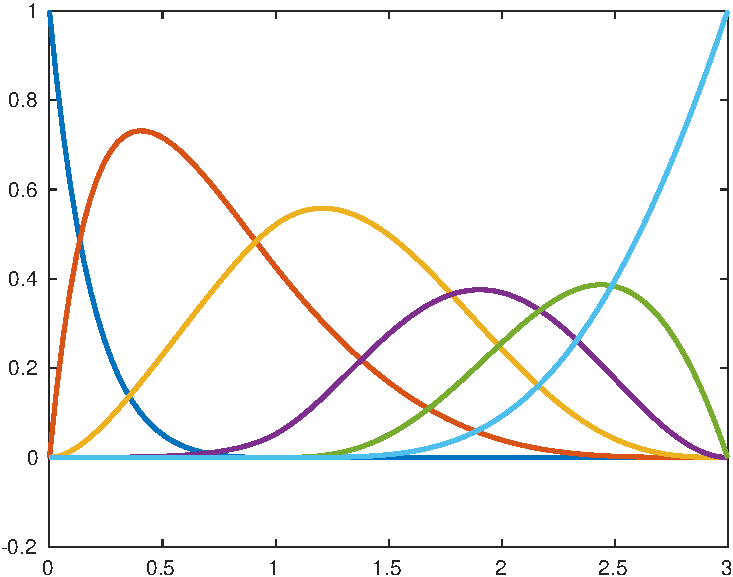
\includegraphics[width=4.5cm]{manual_ex_mdtbspline0}
\end{center}
\vspace*{-0.30cm}
\end{example}

%------------------------------------------------------------------

\subsection{MDTB\_visualization\_spline} \label{sec:matlab-mdtb-visualization-spline}

This function visualizes a spline in (periodic) MDTB-spline form.

\syntax{MDTB\_visualization\_spline(MP, H, cc, n, specs)}

\begin{inputlist}
  \paramitem{MP}{MDTB-spline multi-patch}
  \paramitem{H}{extraction matrix}
  \paramitem{cc}{vector of coefficients}
  \paramitem{n}{number of evaluation points (optional)}
  \paramitem{specs}{pass any number of plot specifications (optional)}
\end{inputlist}

\begin{remark}
\noindent The extraction matrix \texttt{H} should be deduced from the MDTB-spline multi-patch \texttt{MP} and incorporates the smoothness. Each element of the vector \texttt{cc} corresponds to an MDTB-spline basis function. Hence, \texttt{length(cc)} should be equal to \texttt{size(H,1)}. The parameter \texttt{n} is a positive integer scalar. When no value is specified, \texttt{n = 100} is assumed. The parameter \texttt{specs} allows for any number of input arguments, which are passed on to the function \texttt{plot}. We refer the reader to the documentation of \texttt{plot} for all the plotting options.
\end{remark}

\begin{example}
\noindent Create an MDTB-spline multi-patch with smoothness and a vector of coefficients, and then plot the corresponding spline in MDTB-spline form:
\medskip

\pagebreak

\texttt{>> MP = MDTB\_patch\_gpoly([3, 4], [0, 1, 3], [1, 2], [5, 2]);}

\texttt{>> H = MDTB\_extraction(MP, 2);}

\texttt{>> cc = [1, 3, 5, 4, 0, 2];}

\texttt{>> MDTB\_visualization\_spline(MP, H, cc, 100, 'LineWidth', 2);}

\begin{center}
  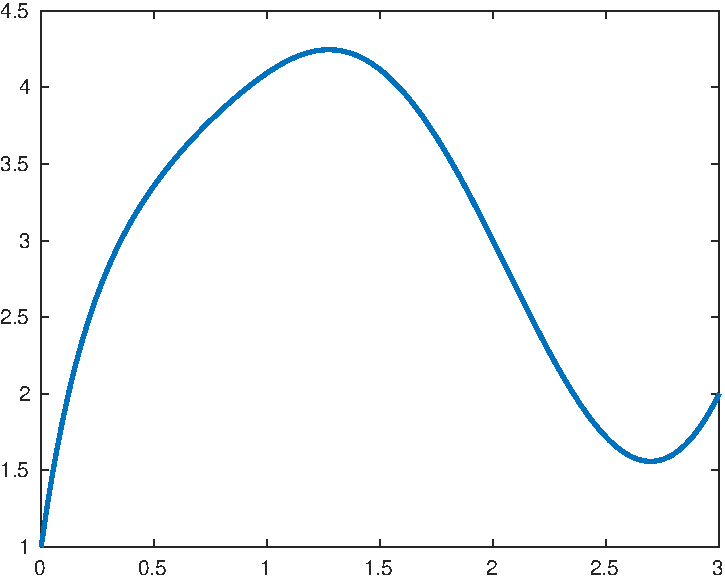
\includegraphics[width=4.5cm]{manual_ex_mdtbspline1}
\end{center}
\vspace*{-0.30cm}
\end{example}

%------------------------------------------------------------------

\subsection{MDTB\_visualization\_curve} \label{sec:matlab-mdtb-visualization-curve}

This function visualizes a spline curve in (periodic) MDTB-spline form.

\syntax{MDTB\_visualization\_curve(MP, H, cc, n, specs)}

\begin{inputlist}
  \paramitem{MP}{MDTB-spline multi-patch}
  \paramitem{H}{extraction matrix}
  \paramitem{cc}{matrix of control points (1D, 2D or 3D)}
  \paramitem{n}{number of evaluation points (optional)}
  \paramitem{specs}{pass any number of plot specifications (optional)}
\end{inputlist}

\begin{remark}
\noindent The extraction matrix \texttt{H} should be deduced from the MDTB-spline multi-patch \texttt{MP} and incorporates the smoothness. Each column of the matrix \texttt{cc} corresponds to an MDTB-spline basis function. Hence, \texttt{size(cc,2)} should be equal to \texttt{size(H,1)}. This matrix consists of $1$, $2$ or $3$ rows, identifying a function, a 2D curve or a 3D curve, respectively. The parameter \texttt{n} is a positive integer scalar. When no value is specified, \texttt{n = 100} is assumed. The parameter \texttt{specs} allows for any number of input arguments, which are passed on to the function \texttt{plot}/\texttt{plot3}. We refer the reader to the documentation of \texttt{plot}/\texttt{plot3} for all the plotting options.
\end{remark}

\begin{example}
\noindent Create an MDTB-spline multi-patch with smoothness and a matrix of 2D control points, and then plot the corresponding 2D spline curve in MDTB-spline form:
\medskip

\texttt{>> MP = MDTB\_patch\_gpoly([3, 4], [0, 1, 3], [1, 2], [5, 2]);}

\texttt{>> Hper = MDTB\_extraction\_periodic(MP, 2, 1);}

\pagebreak

\texttt{>> ccper = [1, 3, 5, 4; 2, 0, 2, 4];}

\texttt{>> MDTB\_visualization\_curve(MP, Hper, ccper, 100, 'LineWidth', 2);}

\begin{center}
  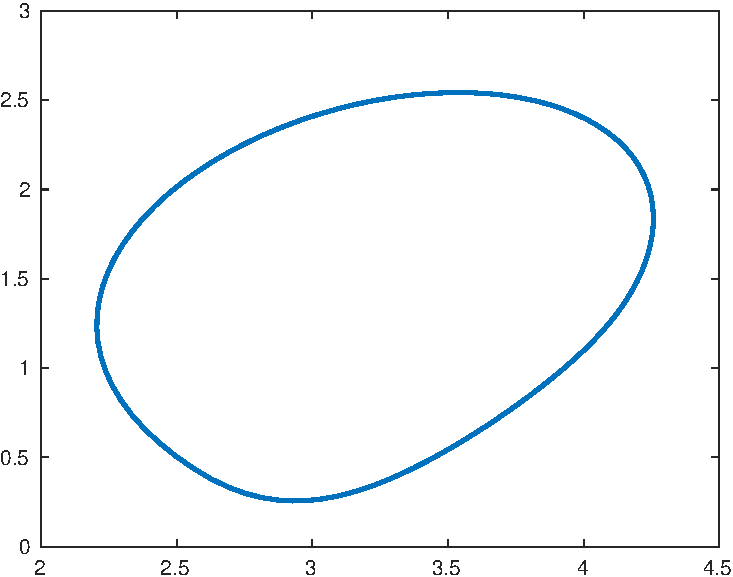
\includegraphics[width=4.5cm]{manual_ex_mdtbspline2}
\end{center}
\vspace*{-0.30cm}
\end{example}

%------------------------------------------------------------------

\subsection{MDTB\_conversion} \label{sec:matlab-mdtb-conversion}

This function converts a spline in (periodic) MDTB-spline form into another (periodic) MDTB-spline form. The conversion is exact when the source and destination MDTB-spline multi-patches with smoothness imply nested spaces. It is assumed that Greville points can be computed.

\syntax{ccd = MDTB\_conversion(MPd, Hd, MPs, Hs, ccs, sh, gl)}

\begin{inputlist}
  \paramitem{MPd}{destination MDTB-spline multi-patch}
  \paramitem{Hd}{destination extraction matrix}
  \paramitem{MPs}{source MDTB-spline multi-patch}
  \paramitem{Hs}{source extraction matrix}
  \paramitem{ccs}{source coefficient vector}
  \paramitem{sh}{shift of the source patch (optional)}
  \paramitem{gl}{global conversion if true (optional)}
\end{inputlist}

\begin{outputlist}
  \paramitem{ccd}{destination coefficient vector}
\end{outputlist}

\begin{remark}
\noindent Different types of TB-spline patches within \texttt{MPs} and \texttt{MPd} may be mixed. The extraction matrix \texttt{Hs} should be deduced from \texttt{MPs} and incorporates the smoothness. Similarly, the extraction matrix \texttt{Hd} should be deduced from \texttt{MPd} and incorporates the smoothness. Each element of the vector \texttt{ccs} corresponds to an MDTB-spline basis function related to \texttt{Hs}. Hence, \texttt{length(ccs)} should be equal to \texttt{size(Hs,1)}. Similarly, each element of the resulting vector \texttt{ccd} corresponds to an MDTB-spline basis function related to \texttt{Hd}. The parameter \texttt{sh} is a real scalar. When no value is specified, \texttt{sh = 0} is assumed. The parameter \texttt{gl} is a boolean scalar. If \texttt{gl} is \texttt{true}, then a global conversion is computed; otherwise, a local patch-wise conversion is computed. The local conversion is more efficient, but requires that the MDTB-spline multi-patches \texttt{MPs} and \texttt{MPd} share the same number of TB-spline patches. Hence, \texttt{length(MPs.P)} should be equal to \texttt{\texttt{length(MPd.P)}}. Moreover, \texttt{MPd} should contain the same break points as \texttt{MPs} for the best local conversion results. When no value is specified, \texttt{gl = true} is assumed.
\end{remark}

\begin{example}
\noindent Create an MDTB-spline multi-patch of multi-degree $(3,4)$ with smoothness and a vector of coefficients; then, raise the multi-degree to $(5,7)$ and compute the coefficients of the new MDTB-spline form:
\medskip

\texttt{>> MPs = MDTB\_patch\_gpoly([3, 4], [0, 1, 3], [1, 2], [5, 2]);}

\texttt{>> Hs = MDTB\_extraction(MPs, 2);}

\texttt{>> ccs = [1, 3, 5, 4, 0, 2];}

\texttt{>> MPd = MDTB\_patch\_gpoly([5, 7], [0, 1, 3], [1, 2], [5, 2]);}

\texttt{>> Hd = MDTB\_extraction(MPd, 2);}

\texttt{>> ccd = MDTB\_conversion(MPd, Hd, MPs, Hs, ccs, 0, false)}

\texttt{ccd =}

\texttt{\ \ Columns 1 through 7}

\texttt{\ \ \ \ 1.0000\ \ \ \ 2.6857\ \ \ \ 3.2379\ \ \ \ 3.6200\ \ \ \ 4.3739\ \ \ \ 4.4464\ \ \ \ 3.7652}

\texttt{\ \ Columns 8 through 11}

\texttt{\ \ \ \ 2.4723\ \ \ \ 1.3250\ \ \ \ 1.0897\ \ \ \ 2.0000}

\medskip
\noindent Now, keep the same multi-degree Tchebycheff structure of the original spline but lower its smoothness, and compute the coefficients of the new MDTB-spline form:
\medskip

\texttt{>> MPe = MPs;}

\texttt{>> He = MDTB\_extraction(MPe, 1);}

\texttt{>> cce = MDTB\_conversion(MPe, He, MPs, Hs, ccs, 0, false)}

\texttt{cce =}

\texttt{\ \ \ \ 1.0000\ \ \ \ 3.0000\ \ \ \ 3.9047\ \ \ \ 4.7632\ \ \ \ 4.0000\ \ \ -0.0000\ \ \ \ 2.0000}

\medskip
\noindent Finally, find an approximation of the original spline using polynomial segments of the same multi-degree $(3,4)$:
\medskip

\texttt{>> MPf = MDTB\_patch\_poly([3, 4], [0, 1, 3]);}

\texttt{>> Hf = MDTB\_extraction(MPf, 2);}

\texttt{>> ccf = MDTB\_conversion(MPf, Hf, MPs, Hs, ccs, 0, false)}

\texttt{ccf =}

\texttt{\ \ \ \ 1.0000\ \ \ \ 3.5162\ \ \ \ 4.7362\ \ \ \ 3.8197\ \ \ \ 0.1696\ \ \ \ 2.0000}
    
\medskip
\noindent Modifying the local Tchebycheff structure does not preserve the exact shape of the original spline, but it forms a reasonable approximation. The approximation can be improved by using locally polynomial spline segments (of uniform degree):
\medskip

\texttt{>> [MPg, rg] = MDTB\_patch\_poly([3, 3, 4, 4], [0, 1/2, 1, 2, 3], 2);}

\texttt{>> Hg = MDTB\_extraction(MPg, rg);}

\pagebreak 

\texttt{>> ccg = MDTB\_conversion(MPg, Hg, MPs, Hs, ccs, 0, false)}

\texttt{ccg =}

\texttt{\ \ Columns 1 through 7}

\texttt{\ \ \ \ 1.0000\ \ \ \ 2.6365\ \ \ \ 3.4343\ \ \ \ 4.2898\ \ \ \ 4.4048\ \ \ \ 3.0828\ \ \ \ 1.4169}

\texttt{\ \ Columns 8 through 9}

\texttt{\ \ \ \ 1.2354\ \ \ \ 2.0000}

\medskip
\noindent Make a visual comparison between the original spline (blue) and the polynomial spline approximation (red):
\medskip

\texttt{>> MDTB\_visualization\_spline(MPs, Hs, ccs, 50, 'LineWidth', 2, ...}

\texttt{>>\ \ \ \ \ \ \ \ \ \ \ \ \ 'Marker', 'o', 'MarkerSize', 10, 'Color', 'blue');}

\texttt{>> hold on;}

\texttt{>> MDTB\_visualization\_spline(MPg, Hg, ccg, 50, 'LineWidth', 2, ...}

\texttt{>>\ \ \ \ \ \ \ \ \ \ \ \ \ 'Marker', '*', 'MarkerSize', 10, 'Color', 'red');}

\texttt{>> hold off;}

\begin{center}
  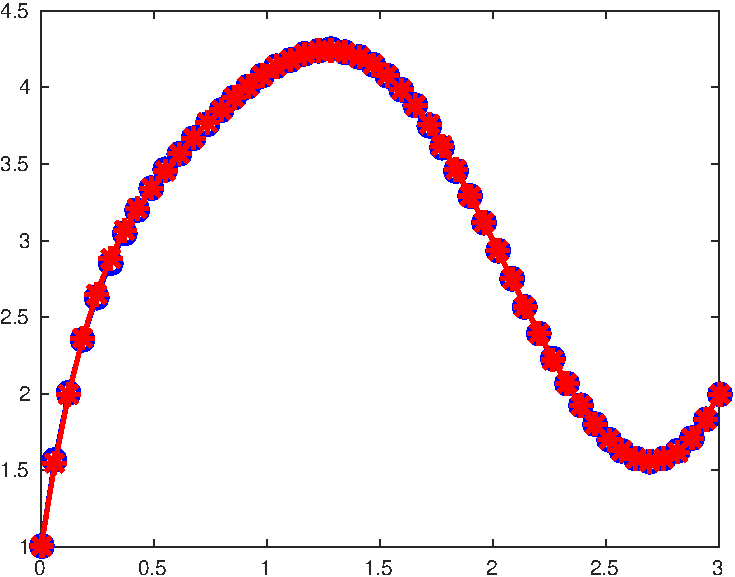
\includegraphics[width=4.5cm]{manual_ex_mdtbspline3}
\end{center}
\end{example}

\end{document}
